\chapter{The CMS experiment}
\label{chap:cms}

\section{Introduction}
With a circumference of 27~km, the Large Hadron Collider (LHC)~\cite{1748-0221-3-08-S08001} at CERN is both the largest and most powerful particle accelerator in the world. The machine is designed to collide hadrons together with sufficiently high energy and frequency to enable stringent tests of the SM at the electroweak energy scale. The ATLAS~\cite{Aad:2008zzm}, ALICE~\cite{Aamodt:2008zz}, CMS~\cite{Chatrchyan:2008zzk} and LHCb~\cite{Alves:2008zz} experiments are situated at four independent locations along the LHC ring, at which the oppositely circulating hadron beams are focused and brought into collision. Each experiment consists of a particle detector apparatus to measure the products of the hadron collisions, where the design of the detector is chosen to facilitate the respective physics programme: ATLAS and CMS are general purpose detectors designed to measure a wide range of physics processes, whereas LHCb and ALICE are more specialised, focusing on flavour physics and heavy-ion physics respectively. 

The measurements presented in this thesis are performed using data collected by the CMS experiment. This chapter serves as an introduction to both the LHC and the CMS detector, and will help the reader understand how the design of these machines enable the predictions of the SM to be accurately probed using high energy hadron collisions. After introducing the operation and design of the machines in sections \ref{sec:lhc} and \ref{sec:cms}, the focus shifts towards the techniques used to reconstruct the collision products in the CMS detector, detailed in \ref{sec:particle_flow}. Here, particular attention is given to the objects which are most relevant for the \Hgg measurements outlined in chapters~\ref{chap:hgg_overview}--\ref{chap:hgg_results}. Following this, the use of Monte-Carlo simulation to accurately predict the behaviour of collision events in the detector is detailed. The chapter finishes with an introduction to machine learning (ML) algorithms, which are becoming an increasing powerful tool in CMS physics analyses.

% concludes by looking at a future operation of the LHC machine, known as the High-Luminosity LHC (HL-LHC)~\cite{}, where the rate of collisions will be increased to approximately five times the nominal value. To accommodate this, many parts of the CMS detector will need to be upgraded. Section \ref{sec:hgcal} details one of the key parts of the upgrade programme known as the high granularity calorimeter (HGCAL)~\cite{}. The application of a Boosted Decision Tree (BDT) algorithm to identify electrons and photons from hadronic objects in the HGCAL Level-1 trigger system is detailed. Finally, a simulation-only study is presented in section \ref{sec:trilinar}, looking at the physics reach of the HL-LHC in terms of the sensitivity to the Higgs boson self coupling from top-associated Higgs boson production.

\section{Large Hadron Collider}\label{sec:lhc}

\begin{figure}[htb!]
  \centering
  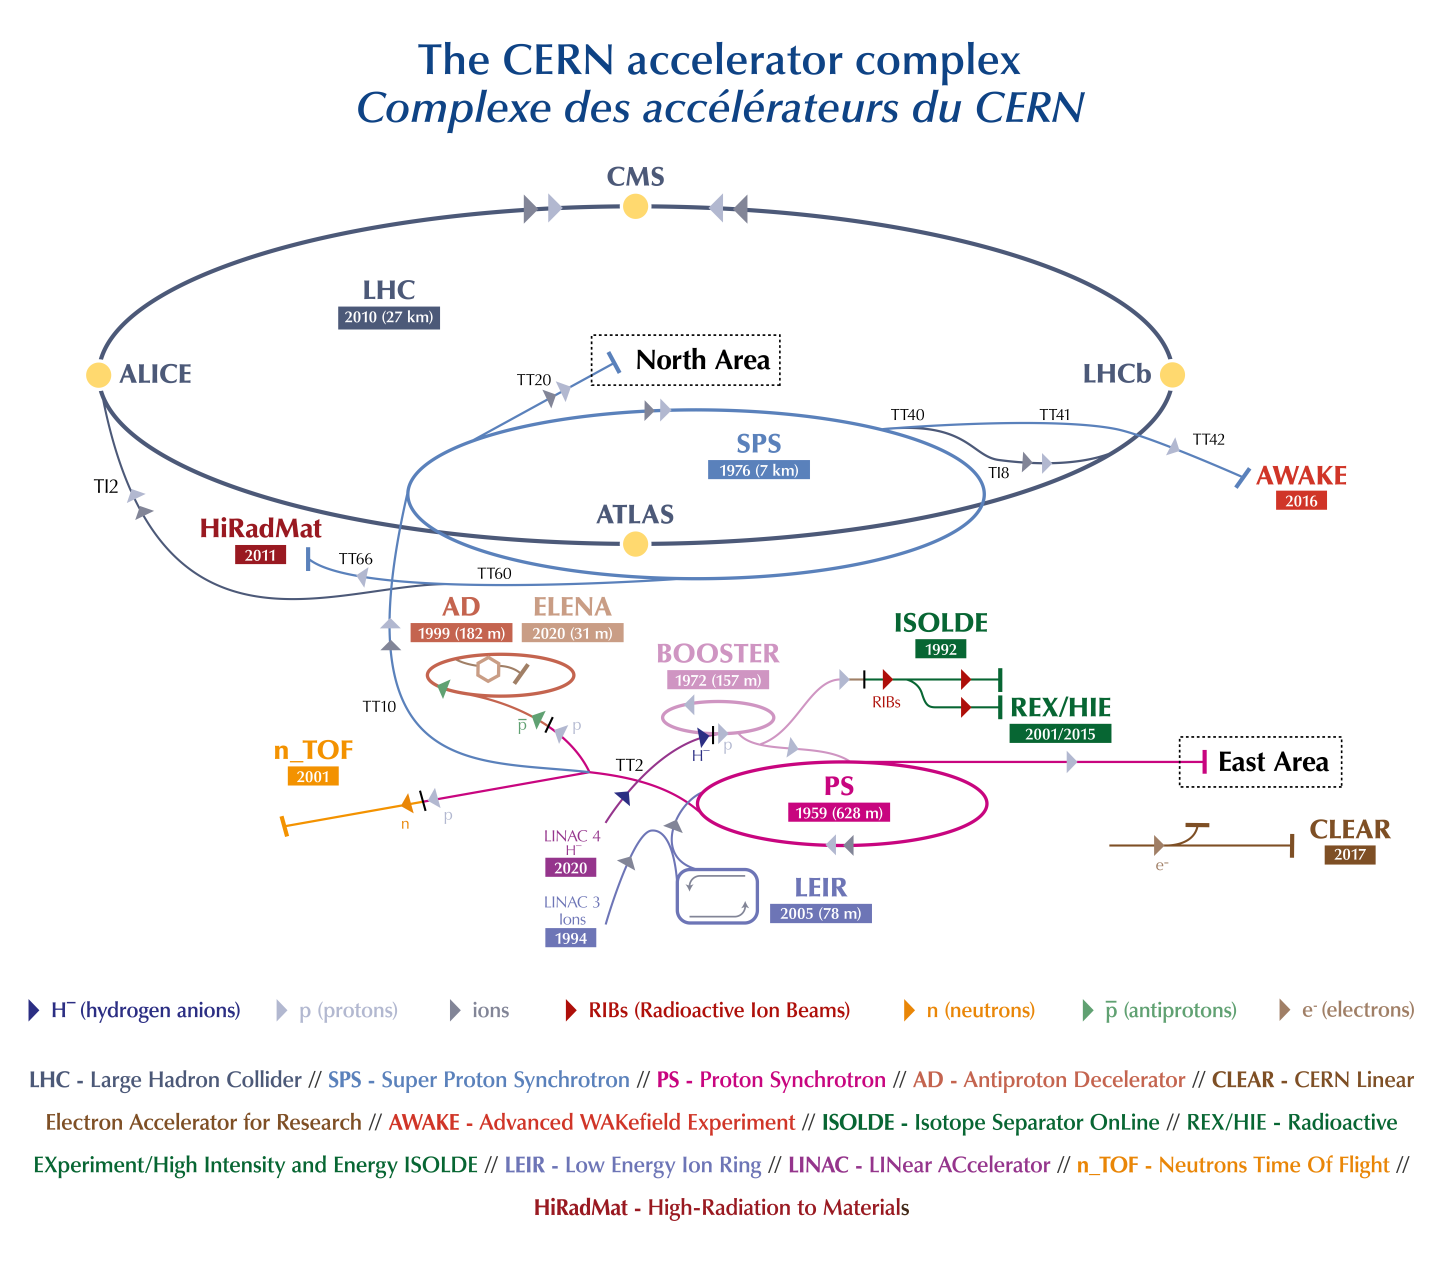
\includegraphics[width=1\textwidth]{Figures/cms/cern_accelerator.png}
  \caption[The CERN accelerator complex]
  {
    An illustration of the CERN accelerator complex, including the four main LHC experiments: ATLAS, ALICE, CMS, and LHCb. The LINAC 2, BOOSTER, PS and SPS are used to sequentially accelerate the proton beams, at which point they are injected into the LHC ring. Diagram is taken from Ref.~\cite{Mobs:2684277}.
  }
  \label{fig:cern_accelerator_complex}
\end{figure}

The LHC is situated 100~m underground the French-Swiss border in the tunnel which previously housed the LEP collider~\cite{lep_design}. Both proton-proton (p-p) collisions and heavy ion collisions are performed, where the former is used for measurements at the electroweak scale such as those presented in this thesis. Therefore p-p collisions will be the focus of this section. A chain of machines, known as the CERN accelerator complex, are used to progressively accelerate protons to higher and higher energies, until they are eventually injected into the LHC ring and brought into collision. The full CERN accelerator complex, including the LHC and its experiments are illustrated in Figure \ref{fig:cern_accelerator_complex}.

Firstly, protons are extracted by stripping electrons from hydrogen atoms using a strong electric field. The protons are sequentially accelerated to an energy of 50~MeV by the Linear Accelerator 2 (LINAC 2), to 1.4~GeV in the BOOSTER, and to 25~GeV in the Proton Synchotron (PS). Here, they are additionally spaced into bunches, with each bunch containing several billion protons. Following this, the bunched beams are fed into the Super Proton Synchotron (SPS), accelerated to an energy of 540~GeV and finally injected into the two concentric LHC beam pipes. The beam travels clockwise in the first pipe, and counter-clockwise in the second, producing two counter-circulating proton beams in the LHC ring. This injection is performed until each beam consists of 2808 proton bunches, with a spacing between them of around 25~ns.

A series of 1,232 super-conducting dipole magnets are located along the LHC ring to keep the beams in a circular orbit. These bending magnets are cooled to a temperature of 1.9~K using superfluid helium. Sixteen radiofrequency (RF) cavities are used to accelerate the beams from 540~GeV to the final beam energy. As the beam energy increases, the magnetic field delivered by the bending magnets is increased accordingly to maintain the circular trajectories of the beams. Currently, the highest energy reached for stable operation is 6.5~TeV per beam, which corresponds to a bending magnetic field of 8.3~T. Quadrapole magnets are then used to focus the protons beams at the four interaction points, where the beams are made to collide every 25~ns with a corresponding centre-of-mass energy of $\sqrt{s}=13$~TeV. Note, this is slightly below the maximum LHC design energy of 14~TeV, which would require an energy of 7~TeV per beam; this is expected to be achieved either during run 3 of the LHC (beginning 2022) or during the High-Luminosity LHC operation\footnote{See chapter~\ref{chap:hllhc}.} (beginning 2027).

\subsection{Luminosity}
The rate of a particular physics process, $R$, in an LHC experiment is governed by the following relation,

\begin{equation}\label{eq:lumi_rate}
    R = \sigma(\sqrt{s}) \cdot \mathcal{L}_{\rm{inst}}
\end{equation}
\noindent
where $\sigma$ is the cross section of the process of interest, and $\mathcal{L}_{\rm{inst}}$ is the instantaneous luminosity of the LHC machine. The cross section depends on the collision centre-of-mass energy, $\sqrt{s}$, such that raising the collision energy can increase the probability of rare, high-energy processes. The instantaneous luminosity depends solely on the beam parameters according to~\cite{1748-0221-3-08-S08001},

\begin{equation}\label{eq:inst_lumi}
    \mathcal{L}_{\rm{inst}} = \frac{n_bN_b^2f_{\rm{rev}}\gamma_r}{4\pi\epsilon_n\beta^*}F,
\end{equation}

\noindent
where $n_b$ is the number of bunches per beam, $N_b$ is the number of particles per bunch, $f_{\rm{rev}}$ is the revolution frequency, $\gamma_r$ is the relativistic gamma factor, $\epsilon_n$ is the normalised transverse beam emittance, $\beta^*$ is the beta-function at the collision point, and $F$ is a reduction factor which accounts for the crossing angle of the beams at the collision point. Ultimately, the exploration of rare events in an LHC experiment requires both high energy and high luminosity.

\begin{figure}[htb!]
  \centering
  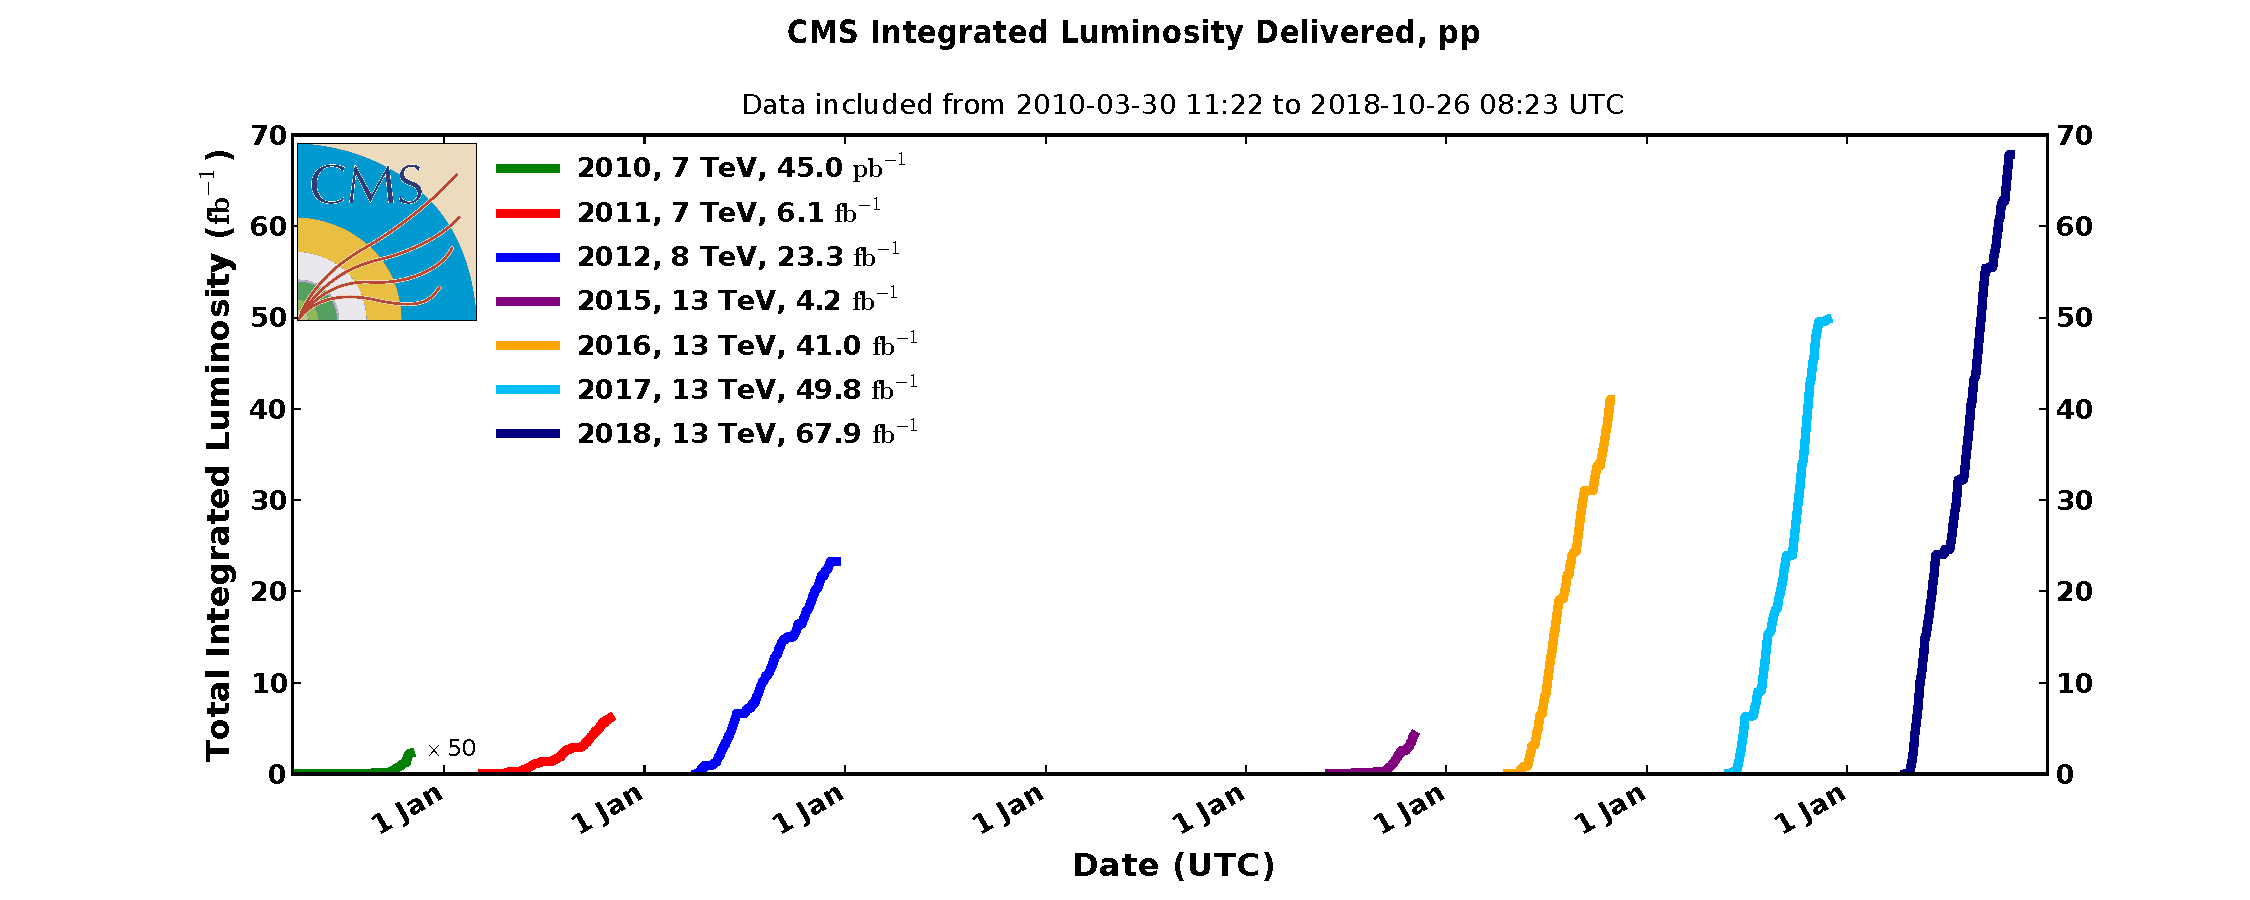
\includegraphics[width=1\textwidth]{Figures/cms/luminosity.pdf}
  \caption[The total integrated luminosity delivered to the CMS experiment]
  {
    The total integrated luminosity delivered to the CMS experiment as a function of time, for each year of operation.
    Figure is taken from Ref.~\cite{CMSLumiPublic}.
  }
  \label{fig:luminosity}
\end{figure}

The LHC was initially designed to run with an instantaneous luminosity of $1\times10^{34}$~cm$^{\rm{2}}$~s$^{\rm{-1}}$. During the 2016-2018 data-taking period this design luminosity was exceeded, eventually levelling at a value of $2 \times 10^{34}$~cm$^{\rm{2}}$~s$^{\rm{-1}}$ for most of the 2018 operation. By integrating the relation in equation \ref{eq:lumi_rate}, we arrive at an expression for the number of events of the process of interest, $N=\sigma\cdot\mathcal{L}$, where $\mathcal{L}$ is the time-\textit{integrated luminosity}, and is a direct measure of the amount of p-p collision data delivered to a collider experiment. Figure~\ref{fig:luminosity} summarises the total integrated luminosity delivered to the CMS experiment throughout its operation. There have been two active phases of the LHC, separated by a shutdown period for upgrades. Run 1 began in 2010 with $\sqrt{s}=7$~TeV, continuing to 2011, such that a total of 6.1~\fbinv of data were collected by CMS at this centre-of-mass energy. In 2012, the energy was increased to $\sqrt{s}=8$~TeV, and a further 23.3~\fbinv of data were collected. This Run 1 dataset was the one used for the Higgs boson discovery~\cite{Aad:2012tfa,Chatrchyan:2012xdj,Chatrchyan:2013lba}. 

Run 2 commenced in 2015 and finished in 2018, where protons were collided with $\sqrt{s}=13$~TeV for the full data-taking period. The increase in instantaneous luminosity (gradient of the lines in Figure \ref{fig:luminosity}) during this period has allowed for an extremely large p-p collision dataset to be accumulated, therefore enabling a large improvement in the statistical precision of the measured processes of interest. The results presented in this thesis use data collected during the 2016-2018 data-taking period. In practice, the CMS experiment operates with a data-taking efficiency of around 90\%, such that the amount of data recorded by the experiment and available for physics analysis, over this period, is approximately 137~\fbinv.

One of the drawbacks of increasing the instantaneous luminosity is the enhancement of \textit{pileup}, defined as the number of additional inelastic p-p collisions for each hard-scattering process of interest. As pileup increases, more sophisticated techniques are required to separate the rare process of interest from the objects originating from pileup interactions. In 2016, the mean number of pileup interactions was 23 per bunch crossing, rising to 32 in both the 2017 and 2018 periods. During the HL-LHC phase of operation, the pileup will increase up to a maximum value of around 200, which poses a major challenge to maintain the current excellent reconstruction performance of the CMS detector.

\section{The CMS detector}\label{sec:cms}
CMS is one of two general purpose particle detectors at the LHC~\cite{Chatrchyan:2008zzk}, located close to the French village of Cessy. It is over 28~m long, 15~m in diameter, and weighs approximately 14,000~tons. The detector is designed to overcome the experimental challenges that arise in a high-energy collision environment with $\mathcal{O}(1000)$ charged particles being produced every 25~ns. This includes a high level of spatial and timing granularity, with many synchronized detector electronic channels, to maintain a sufficiently low occupancy in these conditions. In addition, the detector and front end electronics must be sufficiently radiation-hard to accommodate the high flux of particles.

One of the main goals of the CMS physics programme was the discovery, and is now the measurement of the Higgs boson and its interactions with other particles. Moreover, the programme includes the precise measurement of other rare processes in the SM, and the search for new BSM physics such as supersymmetry or extra dimensions. To achieve these goals, the detector is designed to:

\begin{itemize}
    \item Identify and reconstruct muons with excellent efficiency and precision. This must be achieved over a wide range of muon energies and angles. In addition, the charge of a muon must be ascertained to a high level of accuracy. The reconstruction of muons is central to Higgs boson measurements, specifically in the \Hfl decay channel.
    \item Achieve a good momentum resolution for charged particles, as well as have the ability to locate secondary vertices consistent with originating from $\tau$'s and b quarks.
    \item Measure the energy of electrons and photons with excellent resolution over a wide geometrical coverage. Additionally, the detector is able to isolate photons and electrons efficiently in a high occupancy environment. These characteristics are key to the \Hgg measurement described in chapters \ref{chap:hgg_overview}-\ref{chap:hgg_results}.
    \item Identify sprays of hadrons, known as jets, which originate from the hadronisation of quarks and gluons, and achieve a good dijet mass resolution.
    \item Accurately calculate the missing momentum in an event, which is the key signature of neutrinos or potential BSM particles which do not interact with the detector material.
\end{itemize}

\begin{figure}[htb!]
  \centering
  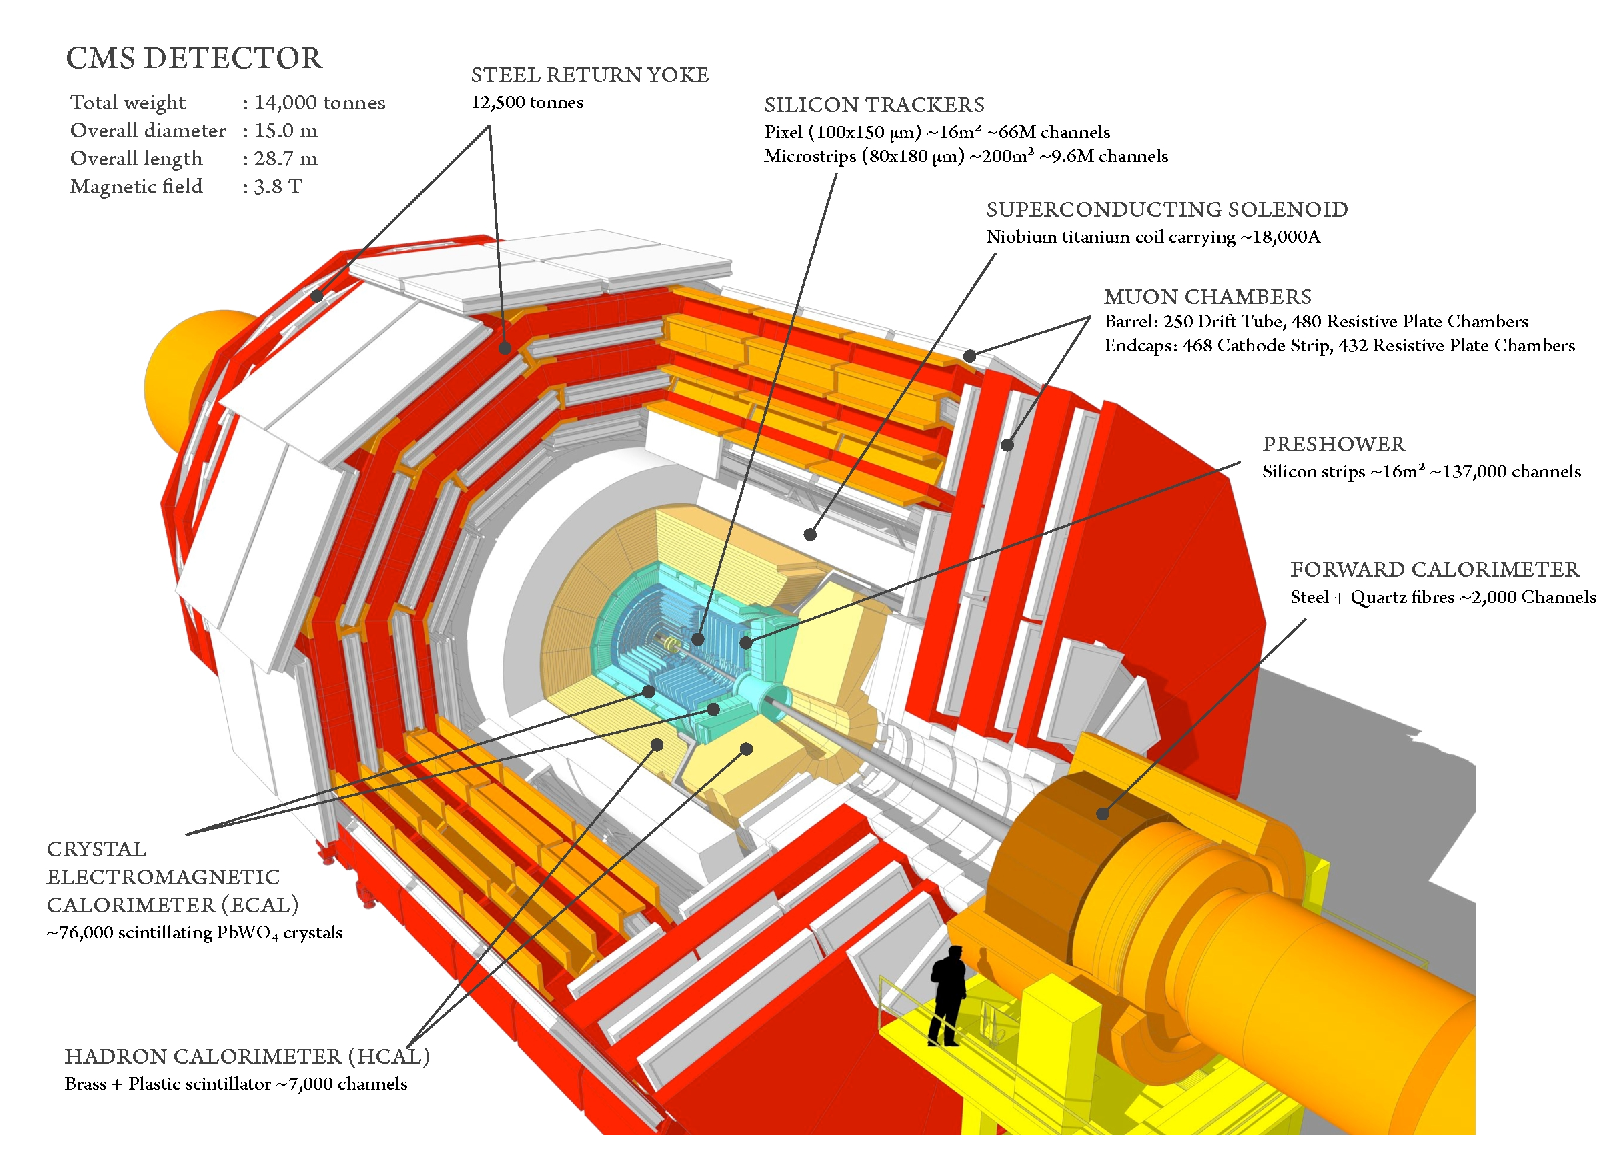
\includegraphics[width=1\textwidth]{Figures/cms/cms_detector.pdf}
  \caption[The CMS detector]
  {
    A schematic of the CMS detector. Part of the detector has been removed so that the layout is visible. Figure is taken from Ref.~\cite{Sakuma_2014}.
  }
  \label{fig:cms_detector}
\end{figure}

A schematic of the CMS detector is provided in Figure~\ref{fig:cms_detector}. The detector consists of a number of components layered around the beam axis, where each component is comprised of a cylindrical \textit{barrel} section and two \textit{endcaps}. At the heart of this (almost) hermetic cylindrical design is the 3.8~T superconducting solenoid magnet, which provides an extremely high bending power for charged particles traversing the inner region of the detector. Within the coil of the 13~m long, 6~m in diameter solenoid lies the silicon tracker (section \ref{sec:cms_tracker}), the homogeneous crystal electromagnetic calorimeter (section \ref{sec:cms_ecal}), and the sampling hadronic calorimeter (section \ref{sec:cms_hcal}), listed in increasing distance from the interaction point. The muon detection system (section \ref{sec:cms_muon}) is embedded within the iron return yoke of the solenoid. This system of subdetectors, and their respective layering, enables the precise reconstruction of the wide range of physics objects produced in hadron collisions.

\subsection{Co-ordinate system}
A right-handed Cartesian co-ordinate system is adopted, centred at the nominal interaction point, such that the $x$-axis points towards the centre of the LHC ring, the $y$-axis points vertically upwards, and the $z$-axis points along the beam pipe in the direction of the counter-clockwise beam. It is more convenient to use a cylindrical co-ordinate system where the direction of an outgoing particle is expressed using the angular quantities: $\phi$ and $\eta$. Here, $\phi \in [-\pi,\pi]$ is defined as the azimuthal angle in the ($x-y$) plane, relative to the $x$-axis. The quantity $\eta$, referred to as the pseudorapidity, is a measure of the polar angle relative to the beam axis, $\theta$, such that,
\begin{equation}
    \eta = - \ln[\tan(\theta/2)].
\end{equation}
Particles with high values of $\eta$ correspond to a direction close to the LHC beam pipe, and are said to be \textit{forward}. The distance measure in the $(\eta,\phi)$ space is defined as $\Delta R = \sqrt{\Delta\eta^2+\Delta\phi^2}$. 

In processes of interest, particles are generally produced with a high momentum in the plane perpendicular to the beam axis. As a result, a useful quantity to characterise a particle is the transverse momentum, $p_T = \sqrt{p_x^2+p_y^2}$, defined as the projection of the particle's total momentum onto this transverse plane. Finally, the missing transverse momentum, \met, is defined as the magnitude of the negative vector sum of particle's momenta in the transverse plane.

\subsection{Tracker}\label{sec:cms_tracker}
The tracker is the innermost component of the CMS detector~\cite{Chatrchyan:2008zzk,Chatrchyan:2014fea}, and is designed to measure the trajectory of charged particles deflected by the 3.8~T magnetic field. The tracker is also able to accurately locate the position of the primary hard scattering interaction vertex, as well as identify secondary interaction vertices which originate from the decay of $\tau$'s or b quarks. 

Being the closest subdetector to the interaction point (IP), the tracker experiences an intense particle flux of $\mathcal{O}(1000)$ particles every 25~ns. As a result, it must simultaneously be able to withstand severe radiation damage, whilst exhibiting excellent spatial and temporal granularity to correctly identify trajectories and attribute them to the correct proton bunch crossing. To achieve such levels of granularity, a complicated system of power-dense on-detector electronics are required, which in-turn require an efficient cooling system to obviate overheating. These technical requirements directly oppose the need to limit the amount of material in the tracker to mitigate unwanted interactions, such as bremsstrahlung and photon conversions. Effectively, a larger amount of material in the tracker leads to a worse energy measurement in the electromagnetic calorimeter, directly impacting the sensitivity of the \Hgg analysis. Ultimately, to satisfy the requirements of radiation hardness and granularity, whilst keeping the material budget to a minimum, the tracker is composed entirely of silicon detector technology.

\begin{figure}[htb!]
  \centering
  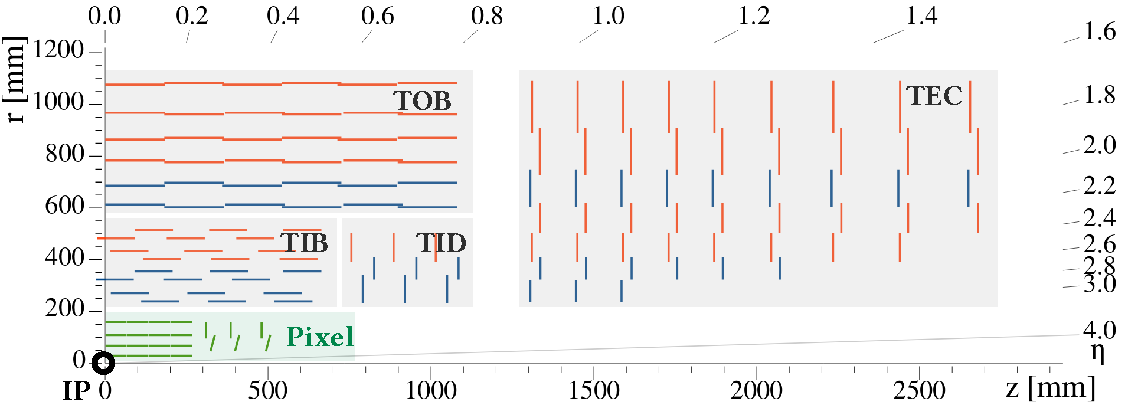
\includegraphics[width=1\textwidth]{Figures/cms/tracker.pdf}
  \caption[The CMS silicon tracker]
  {
    A diagram showing one quarter of the CMS tracker in the $r$-$z$ view, where $r$ is a measure of the radial distance in the ($x$-$y$)-plane. The pixel detector, closest to the interaction point (IP, black circle) is shown in green. The sections of the silicon strip tracker (TIB, TID, TOB, TEC) are also shown, where the red and blue lines signify one-sided and two-sided strips respectively. Figure has been adapted from the original in Ref.~\cite{CERN-LHCC-2017-009}.
  }
  \label{fig:cms_tracker}
\end{figure}

Figure \ref{fig:cms_tracker} shows one quarter of the CMS tracker, where the full tracker layout is symmetric about the $r$ and $z$-axes. A pixel detector is located closest to the beampipe. The original pixel detector was designed to operate for ten years at a maximum instantaneous luminosity of $1\times10^{34}$~\lumi, and consisted of three barrel layers at radii of 44, 73, and 102~mm, and two endcap disks at distances of 345 and 465~mm from the IP. To accommodate the enhancement of the LHC instantaneous luminosity, an upgraded pixel detector was installed during the end-of-year technical stop of the LHC in 2016/2017~\cite{CMS:2012sda}. The upgraded detector lies closer to the beampipe with \textit{four} barrel layers at radii of 29, 68, 109, and 160~mm, and \textit{three} endcap disks at distances of 291, 396, and 516~mm from the IP. This enables the measurement of four high precision space points (hits) on each charged particle trajectory, over the pseudorapidity range: $|\eta|<2.5$. Additionally, the upgrade brings an improved performance at higher rates, increased radiation tolerance and offers more robust tracking. The upgraded pixel detector consists of approximately 124~million individual silicon pixels, each of size $100$~$\mu$m~$\times$~$150$~$\mu$m, covering a total area of approximately 1.9~m$^2$. This results in a spatial resolution of around 10~$\mu$m in the transverse ($r$-$\phi$) direction and around 20~$\mu$m in the longitudinal ($z$) direction.

%Whilst, these improvements have a sizeable impact for analyses that rely on the efficient identification of secondary vertices e.g. \Hbb,  the impact on the \Hgg analysis is small.
Beyond a radius of 200~mm, the reduced particle flux allows for the use of silicon strip detectors. The CMS strip tracker consists of three sub-systems. The Tracker Inner Barrel and Disks (TIB/TID) contains four layers of $320$~$\mu$m thick silicon strip sensors in the barrel, supplemented by three disks of the same width at each end. The Tracker Outer Barrel (TOB) encompasses the TIB/TID, extending out to a radius of 1200~mm from the beam pipe, and $\pm$1180~mm in the $z$-direction. It consists of six $500$~$\mu$m thick layers, positioned with their strips parallel to the beam axis. Beyond this $z$-range, the Tracker Endcaps (TECs) extend out to $\pm$2820~mm in $z$, providing a pseudorapidity coverage of $|\eta|<2.4$. Each TEC is composed of 9 disks, carrying as many as seven rings of silicon strip sensors. 

Each silicon strip sensor provides a one-dimensional measurement in $\phi$ of a point along a charged particles trajectory. In addition, the first two layers of the TIB/TID and the TOB, as well as the first, second and fifth rings of the TEC are supplemented with a second strip sensor to provide a measurement of a second spatial co-ordinate: $z$ in the barrel and $r$ in the disks. All in all, the CMS strip tracker has a total of 9.3 millions strips, corresponding to 198~m$^2$ of active silicon.

Charged particles follow helical trajectories in the solenoidal field. By making several precise measurements of hits in both the pixel and strip tracker systems, these charged particle trajectories (tracks) can be reconstructed (see section \ref{sec:particle_flow}). In total, approximately nine hits are measured in the range $|\eta|<2.5$. The momentum of the outgoing particle is then inferred from the curvature of the track, with a resolution of 2\% for high $p_T$ (100~GeV) charged particles up to $|\eta|\approx1.5$. This momentum resolution worsens as a function of charged particle $p_T$, as the curvature of the track decreases. All tracks are extrapolated back to a common point of origin, to identify the primary hard-scattering vertex and any secondary interaction vertices. The performance of this vertex location is driven by the excellent longitudinal resolution of the pixel detector.

\subsection{Electromagnetic calorimeter}\label{sec:cms_ecal}
The electromagnetic calorimeter (ECAL)~\cite{Chatrchyan:2008zzk,Benaglia:1632384,CMS:1997ysd} is used to reconstruct the energy of electromagnetic showers originating from electrons and photons, and therefore is the key sub-detector in the \Hgg analysis. The overall structure of the CMS ECAL is shown in Figure~\ref{fig:cms_ecal}. 

\begin{figure}[htb!]
  \centering
  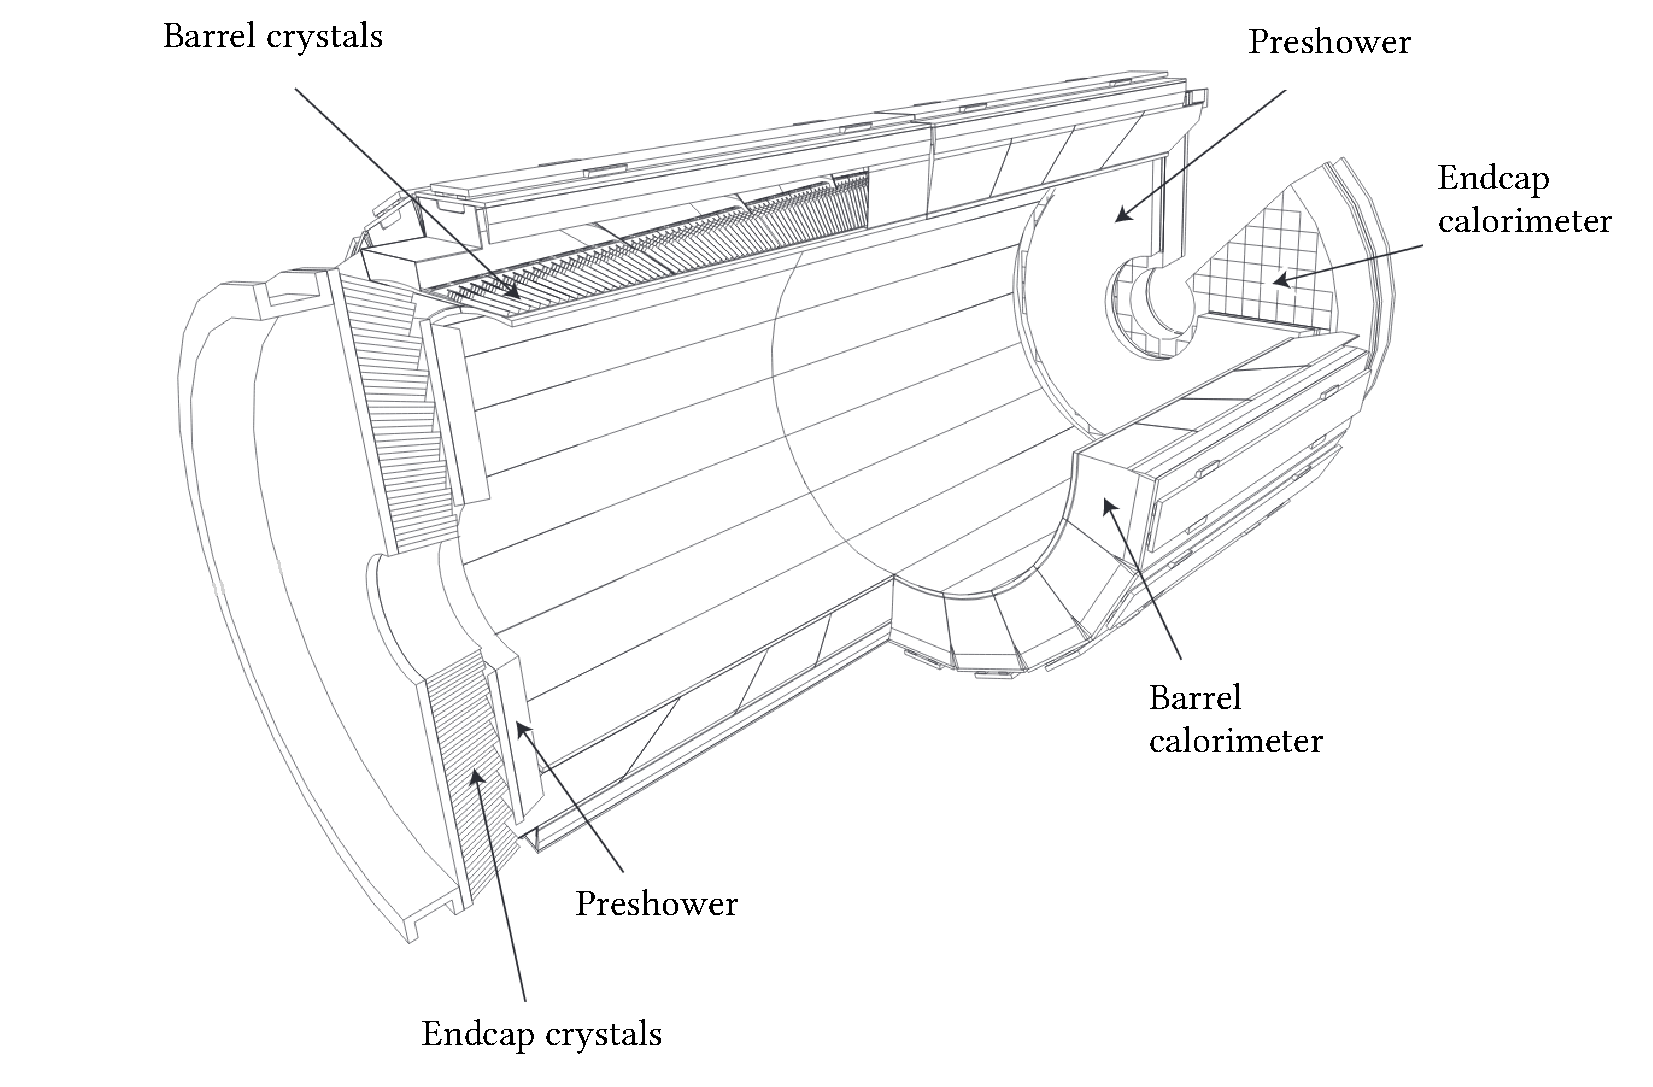
\includegraphics[width=1\textwidth]{Figures/cms/ecal.pdf}
  \caption[The CMS electromagnetic calorimeter]
  {
    A schematic of the CMS ECAL. The tracker and LHC beampipe have been removed from the diagram, in addition to a section of the ECAL, for clarity. Figure has been adapted from that shown in Ref.~\cite{Chatrchyan:2008zzk}.
  }
  \label{fig:cms_ecal}
\end{figure}

The ECAL is a homogeneous calorimeter consisting of 75,848 lead-tungstage (PbWO$_4$) scintillating crystals. It is comprised of the ECAL barrel (EB) section, covering the pseudorapidity region, $|\eta|<1.48$, and two ECAL endcaps (EE), which extend the coverage up to $|\eta|<3.0$. The barrel and endcaps are separated by a transition region, $1.44<|\eta|<1.57$, in which electromagnetic showers cannot be reconstructed. 

When photons and electrons interact with ECAL crystals, they produce scintillation light which is collected by photo-sensors to measure the energy of the incident particle. The choice of PbWO$_4$ is made due to the following properties of the material:
\begin{itemize}
    \item Short radiation length, defined as the mean distance over which an electron loses all but $1/e$ of its energy due to bremsstrahlung, of approximately $X_0=0.89$~cm. This means the longitudinal extension of the electromagnetic shower is kept to a reasonable level.
    \item Narrow Moli\`ere radius, defined as the average radius containing on average 90\% of a shower's total energy deposit, of $r_M=2.19$~cm. This means the lateral extension of the electromagnetic shower is kept to a reasonable level.
    \item Fast response time, such that approximately 80\% of the total scintillation light is emitted by the crystals in  25~ns. This is necessary so that the majority of the energy is collected before the next proton bunch crossing.
    \item Hard radiation tolerance.
\end{itemize}

\noindent
The crystals are arranged in a \textit{quasi}-projective geometry, such that their axis makes a small angle (3$^\circ$) with the vector pointing directly from the nominal IP. This ensures no particle trajectories are completely aligned with the cracks between crystals and therefore a decent fraction of all electromagnetic showers are contained within the crystals. The EB (EE) crystals are $\sim$26 ($\sim$25)~$X_0$ long, meaning that electromagnetic showers up to an energy of approximately 500~GeV are fully contained within the ECAL. The front-face cross section of the EE (EB) crystals are $2.2\times2.2$~cm$^{\rm{2}}$ ($2.86\times2.86$~cm$^{\rm{2}}$); this size is comparable to the Moli\`ere radius, and therefore provides a handle on the shape of the electromagnetic shower which can subsequently be used for photon/electron identification. In the current CMS ECAL, the crystals are arranged in a single layer. A future upgrade of the calorimeter endcaps, known as the HGCAL (section \ref{sec:hgcal}), will also exhibit longitudinal segmentation, and therefore provide granular measurements of the electromagnetic shower in the direction of propagation.

One of the disadvantages of PbWO$_4$ is the relatively low light yield, which demands the use of photo-sensors with internal amplification inside the CMS solenoidal magnetic field. Silicon avalanche photodiodes (APDs) operating with an amplification factor of around 50, and vacuum photo-triodes (VPTs) operating with an amplication factor of around 10, are used in the EB and EE, respectively. Both produce roughly 4,500 photo-electrons per GeV, which are subsequently digitised using a 12-bit analog-to-digital converter (ADC), and stored as discrete amplitude measurements in a buffer. For each crystal, ten consecutive amplitude measurements are stored. If the event is deemed of interest and a trigger (section \ref{sec:trigger}) is received, the ten measurements pass to the off-detector electronics, where the amount of energy deposited in the crystal is inferred from the pulse shape.

An additional subdetector, referred to as the preshower detector (ES), is mounted in front of each endcap, providing a coverage of the pseudorapidity region: $1.65<|\eta|<2.6$. The ES is a 20~cm thick sampling calorimeter composed of two alternating layers of lead (to initiate the electromagnetic showers from incoming photons and electrons), and silicon strips (to measure the deposited energy and the transverse shower profile). The main aim of the ES is to distinguish neutral pions ($\pi^0$), from true photons in this $\eta$ range. 

\subsubsection{Electromagnetic shower energy reconstruction}
The total width of the Higgs boson, $\Gamma^H$, is many orders of magnitude smaller than it's mass ($\sim$4~MeV in the SM). This means the width of the Higgs boson decay products invariant mass distribution is entirely driven by the experimental resolution. Consequently, in the case of the \Hgg analysis, the sensitivity is driven by the ECAL energy resolution.

The intrinsic energy resolution of the ECAL crystals is modelled according to,
\begin{equation}
    \Big(\frac{\sigma}{E}\Big)^2 =  \Big(\frac{S}{\sqrt{E}}\Big)^2 + \Big(\frac{N}{E}\Big)^2 + C^2,
\end{equation}
\noindent
where $S=2.8\%$ is the stochastic term, $N=12\%$ is the noise term, and $C=0.3\%$ is the constant term, whose values have been derived using test beam data~\cite{Chatrchyan:2008zzk}. The energy, $E$, is expressed in units of GeV, and corresponds to the sum of energy in a $5\times5$ array of ECAL crystals. The energy resolution can be improved using a series of corrections, described below.

A typical photon or electron shower is spread over many ECAl crystals. To encompass the energy deposited in the ECAL, a dynamic clustering algorithm is applied (section \ref{sec:particle_flow}). Here, clusters are extended in the $\phi$-direction to form superclusters (SC), which improves the containment for showers that undergo photon conversions or bremsstrahlung in the material upstream of the ECAL. The reconstructed photon or electron energy, $E_{e,\gamma}$, is calculated according to the following equation,
\begin{equation}
    E_{e,\gamma} = F_{e,\gamma} \cdot E_{\rm{SC}} = F_{e,\gamma} \cdot \big[ G(\eta) \cdot \sum_i (C_i \cdot S_i(t) \cdot A_i) + E_{\rm{ES}} \big],
\end{equation}
\noindent
where the index, $i$, iterates over crystals in the SC. The individual channel amplitudes, $A_i$, are multiplied by a time-dependent crystal response correction, $S_i(t)$, and a channel calibration constant, $C_i$, before being summed and multiplied by the global ADC to GeV absolute energy scale factor, $G(\eta)$. Showers in the EE are supplemented with the energy measured in the preshower detector, $E_{\rm{ES}}$. Finally, the energy of the SC, \Eraw, is corrected by applying a multivariate regression, $F_{e,\gamma}$, separately for photons~\cite{Khachatryan:2015iwa} and electrons~\cite{Khachatryan:2015hwa}. More detail of the photon energy regression is provided in the following chapter when the \Hgg analysis is introduced. The impact of these energy corrections is illustrated in Figure \ref{fig:shower_energy_reconstruction}.

The final energy resolution after corrections is shown as a function of $\eta$ for \Zee electrons in data (blue) and simulation (red) in Figure \ref{fig:ecal_energy_resolution}. In the simulation, the ECAL conditions are set to reflect the status of the detector after collecting an integrated luminosity of 25~\fbinv in 2017. A resolution of around 1.5\% is observed in data for low bremsstrahlung electrons ($\RNINE<0.94$) up to an $|\eta|=1$, rising to around 3\% towards the edge of the EB, and up to 4\% in the EE. High bremsstrahlung electrons have a worse resolution of about 2-3\% up to $|\eta|=1$, 3-4\% up to $|\eta|=1.44$, and up to 5\% in the EE\footnote{As electron and photons showers are practically indistinguishable, the photon energy resolution in \Hgg decays is approximately the same, with low bremsstrahlung electrons mapping to unconverted photons, and high bremsstrahlung electrons mapping to photons undergoing a conversion to $e^+e^-$ pairs in the tracker.}. The worse energy resolution in the EE compared to the EB is a direct consequence of the higher radiation dose in the forward region, which affects the crystal transparency.

\begin{figure}[htb!]
  \centering
  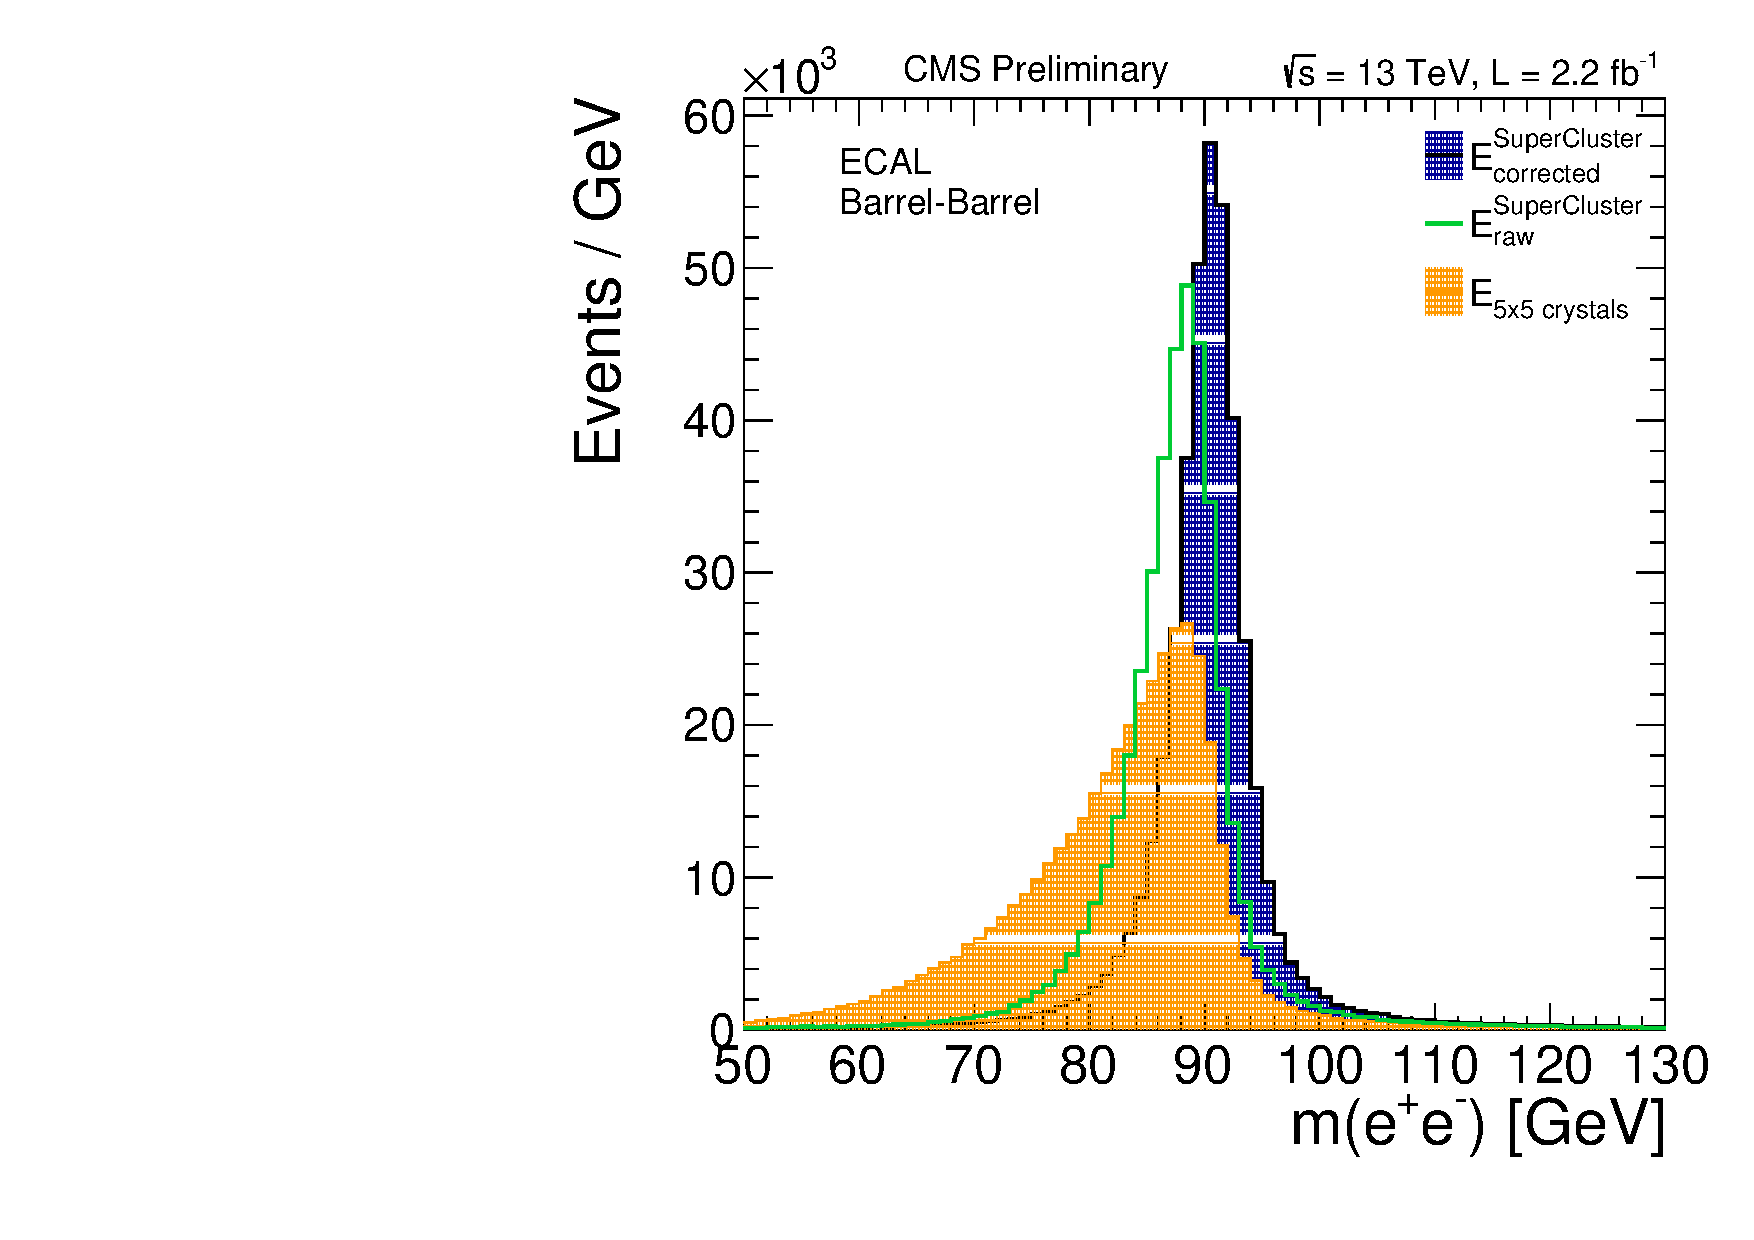
\includegraphics[width=.49\textwidth]{Figures/cms/zee_mass_bb.pdf}
  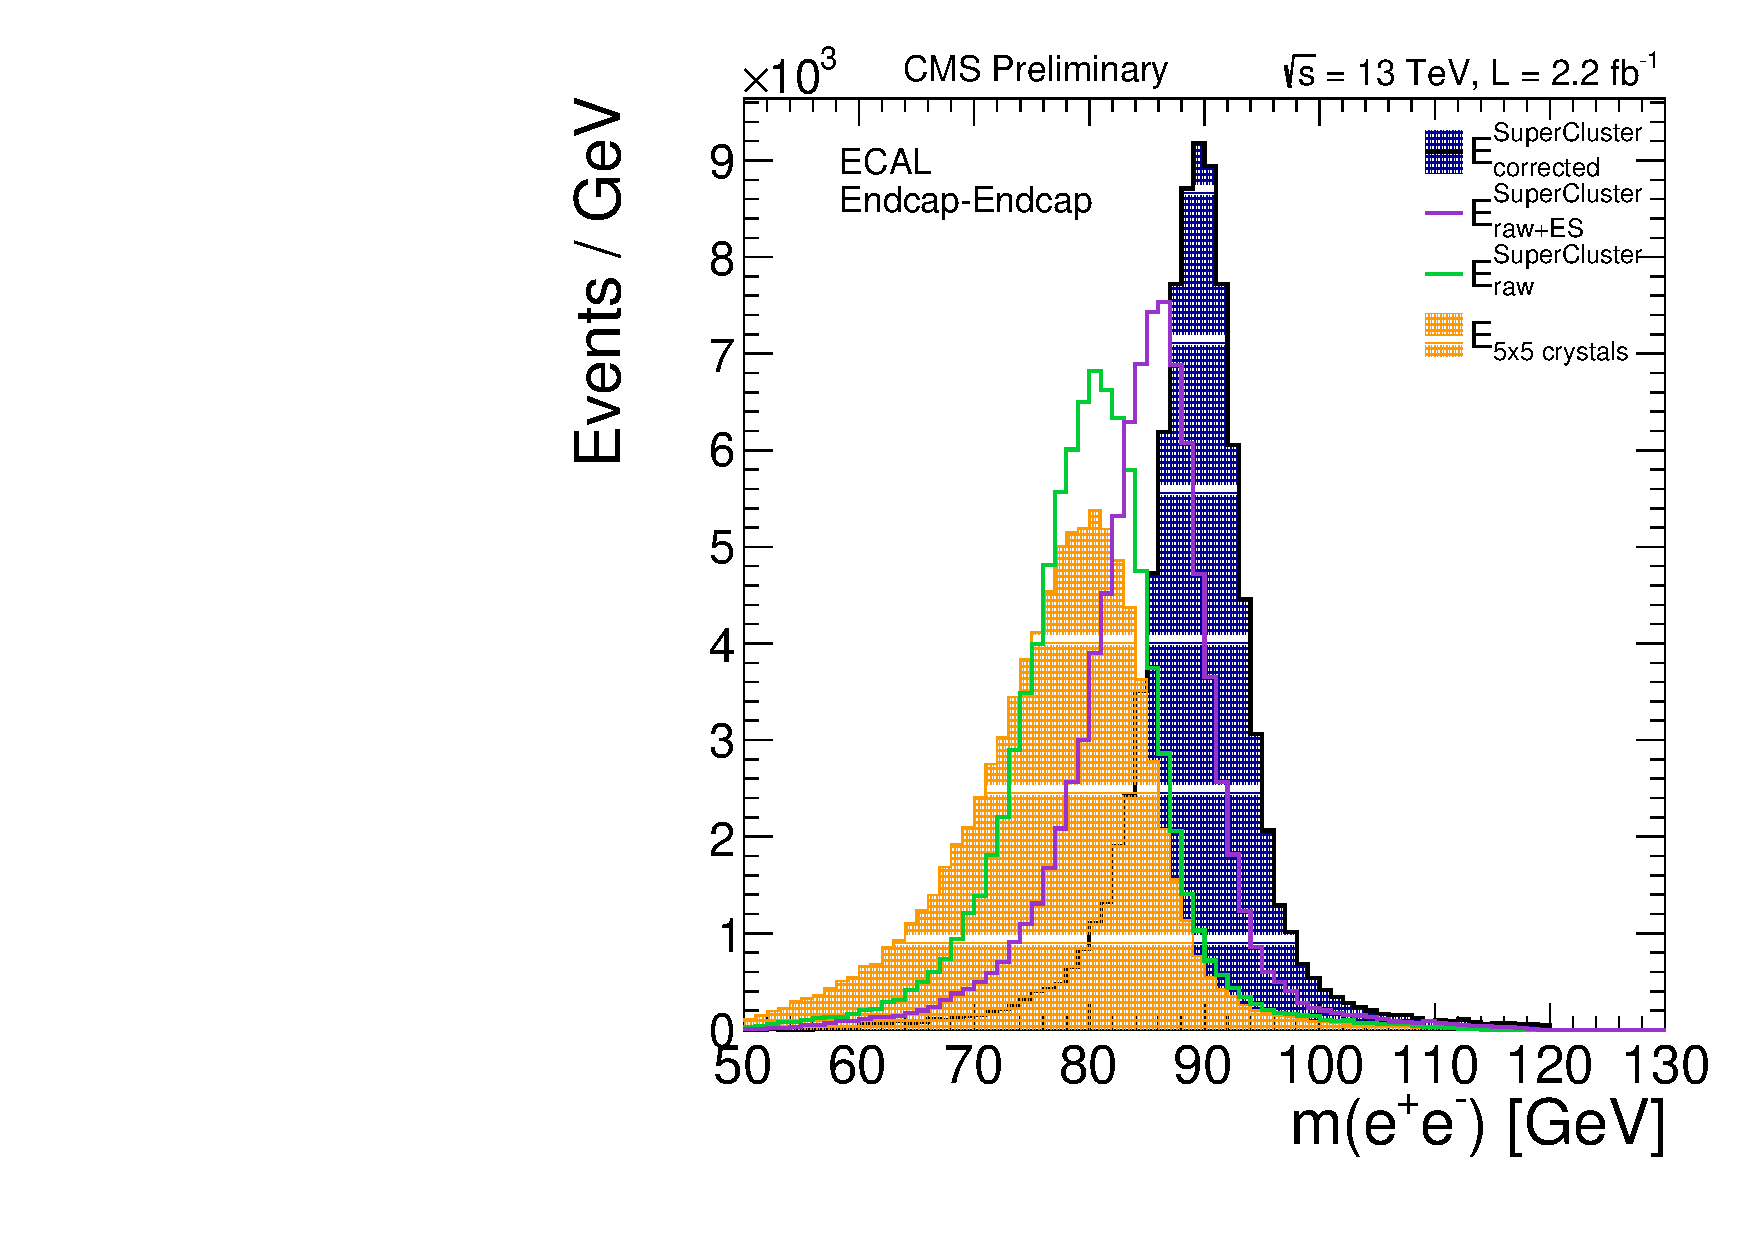
\includegraphics[width=.49\textwidth]{Figures/cms/zee_mass_ee.pdf}
  \caption[Impact of the shower energy reconstruction]
  {
    Improvements to the ECAL energy reconstruction, illustrated using the invariant mass distribution of electron pairs from \Zee events. The left (right) plot shows electron pairs reconstructed in the EB (EE). The yellow histogram uses the simple energy sum over the $5\times5$ array of ECAL crystals. The green line uses the supercluster energy after applying the clustering algorithm, and the purple line in the EE plot also includes the energy deposited in the ES detectors. Finally, the blue histogram uses the energy after all corrections are applied, including the multivariate regression. The data shown was collected during the 2015 period. Figure is taken from Ref~\cite{CMS-DP-2015-057}.
  }
  \label{fig:shower_energy_reconstruction}
\end{figure}

\begin{figure}[htb!]
  \centering
  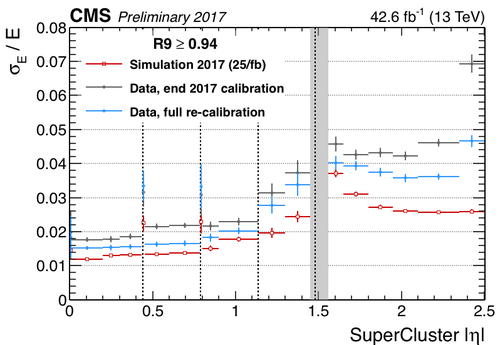
\includegraphics[width=.49\textwidth]{Figures/cms/2017_resolution_highR9.png}
  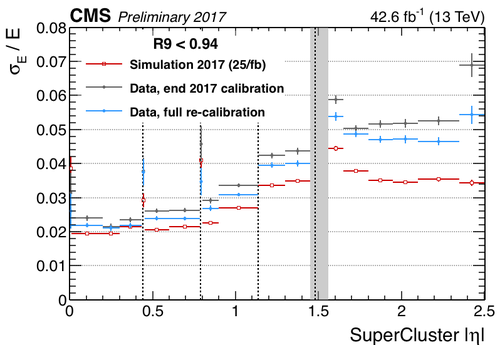
\includegraphics[width=.49\textwidth]{Figures/cms/2017_resolution_lowR9.png}
  \caption[ECAL energy resolution in 2017 data]
  {
    ECAL energy resolution as a function of $\eta$ for electrons from \Zee decays. Both the EB and EE are shown, separated by the transition region (shaded grey). The resolution is plotted for 2017 data after two calibrations: the blue points correspond to the full calibration where the all corrections are applied, whilst the black points represent a calibration in which only the time-dependent effects are corrected for. Also shown is the resolution for simulated \Zee events in red, where the simulation reflects the status of the ECAL after collected 25~\fbinv of data in 2017. The left plot corresponds to low bremsstrahlung electrons ($\RNINE>0.94$), and the right plot to high bremsstrahlung electrons ($\RNINE<0.94$), where the variable \RNINE is defined in table~\ref{tab:photon_variables}. Figure is taken from Ref~\cite{CMS-DP-2018-015}.
  }
  \label{fig:ecal_energy_resolution}
\end{figure}

\subsection{Hadronic calorimeter}\label{sec:cms_hcal}
Quarks and gluons produced in the proton collisions hadronise in the detector, resulting in collimated sprays of particles known as jets. The CMS hadronic calorimeter (HCAL)~\cite{Chatrchyan:2008zzk,CMS:1997xji} is used to measure the position and energy of hadrons in jets. This is especially important for neutral hadrons which leave no track in the silicon tracker, and deposit little energy in the ECAL. Additionally, the HCAL is required for the reconstruction of the \met. The layout of the HCAL for one quarter of the CMS detector is displayed in Figure \ref{fig:cms_hcal}.

\begin{figure}[htb!]
  \centering
  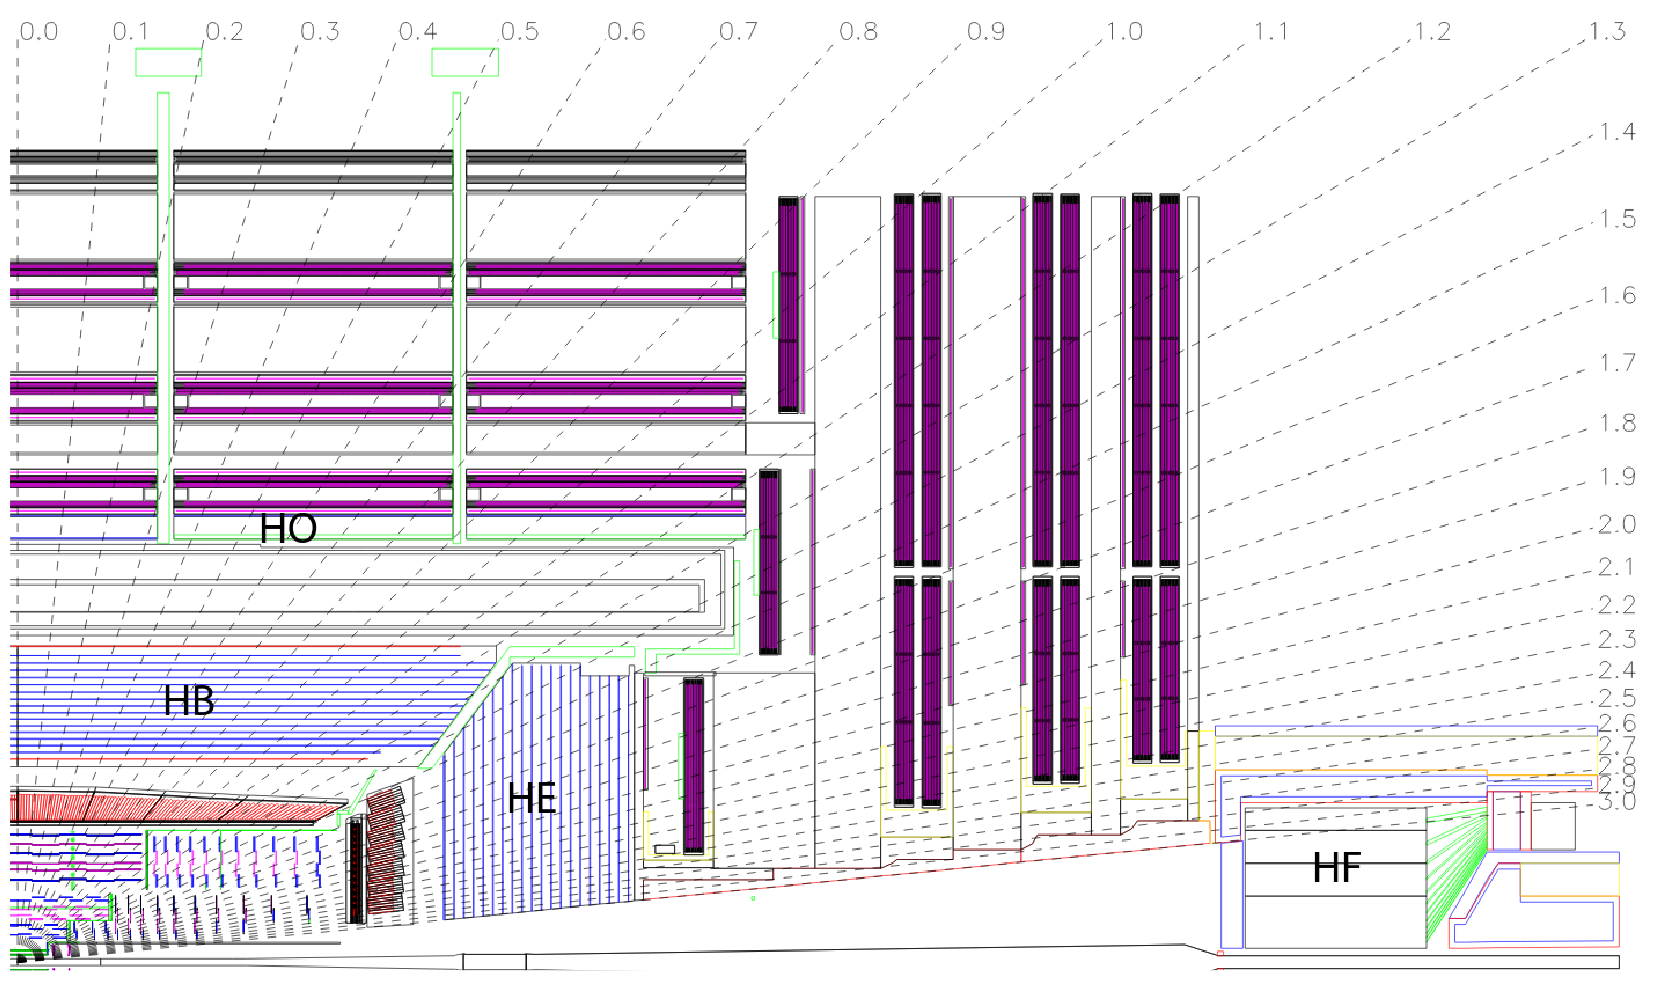
\includegraphics[width=.9\textwidth]{Figures/cms/hcal.pdf}
  \caption[The CMS hadronic calorimeter]
  {
    A schematic showing one quarter of the CMS detector. The dashed lines indicate lines of constant pseudorapidity. The locations of the HB, HO, HE and HF components of the HCAL are shown. Figure is taken from Ref.~\cite{Chatrchyan:2008zzk}.
  }
  \label{fig:cms_hcal}
\end{figure}

The HCAL is a sampling calorimeter consisting of absorber plates made from brass or steel, interleaved with active layers of plastic scintillator. Hadrons traversing the HCAL, shower due to nuclear interactions. Light produced in the scintillator material from these showers is read out by wavelength-shifting plastic fibres, and is used to infer the energy of the incident hadron. It is important that the shower is fully contained to make an accurate measurement of the hadron energy. The HCAL is split up into four components:

\begin{itemize}
    \item The barrel (HB) has coverage up to $|\eta|=1.3$, and consists of 18 identical azimuthal wedges in both the $+z$ and $-z$ directions from the IP. The scintillator in each wedge is divided into 16 $\eta$-sectors, resulting in a spatial granularity of $\Delta\eta\times\Delta\phi=0.087\times0.087$. The HB is confined radially from the outer-edge of the EB at $r=1.77$~m to the inner-coil of the CMS solenoid magnet at $r=2.95$~m. This corresponds to a depth of between 5.8 and 10.6 nuclear interaction lengths ($\lambda_I$), increasing as a function of $\eta$. Here, $\lambda_I$ is a property of the material defined as the mean distance a hadron travels before undergoing an inelastic nuclear interaction.
    \item To ensure hadronic showers in the central region are fully contained, an outer calorimeter (HO) is placed outside of the solenoid. This component treats the solenoidal coil as the absorber, and uses the same active scintillator as the HB, extending the minimum depth to 11.8~$\lambda_I$.
    \item The endcap (HE) calorimeters cover the pseudorapidity range: $1.3<|\eta|<3$. They are designed to be particularly radiation-hard due to the increased particle flux at high $\eta$. The spatial granularity is equivalent to the HB for $|\eta|<1.6$, reducing to $\Delta\eta\times\Delta\phi=0.17\times0.17$ for higher pseudorapidities. In the HE, the minimum depth is 10$~\lambda_I$.
    \item Additional forward calorimeters (HF) are placed 11.2~m from the IP, and extend the coverage up to $|\eta|=5.2$. The particle flux in this region is extremely high, resulting in a very hostile environment; at the design luminosity approximately 800~GeV per p-p collision is deposited in the two HF, compared to only 100~GeV across the rest of the detector. To withstand this extremely high radiation dose, steel-quartz fibres are chosen as the active material, encompassed by a steel absorber structure. Charged particles in the shower emit Cherenkov light in the fibres, which is read by photo-multiplier tubes. Ultimately, the HF are important for the measurement of forward jets, such as those produced in VBF production, and for making the overall HCAL structure as hermetic as possible for the \met reconstruction.
\end{itemize}

\subsection{Muon chambers}\label{sec:cms_muon}
Muons traverse the CMS calorimeters with few interactions. A dedicated muon tracking system~\cite{Chatrchyan:2008zzk,Chatrchyan:2013sba} is positioned furthest from the IP, built into the steel return yoke structure outside the solenoid magnet. Using a combination of information from the innermost silicon tracker and the muon tracking system, CMS is able to accurately identify muons, infer their charge, and measure their energy with excellent resolution. The muon tracking system is comprised of three different gaseous particle detector technologies, where the layout is shown for one quarter of the CMS detector in figure~\ref{fig:cms_muon}. 

\begin{figure}[htb!]
  \centering
  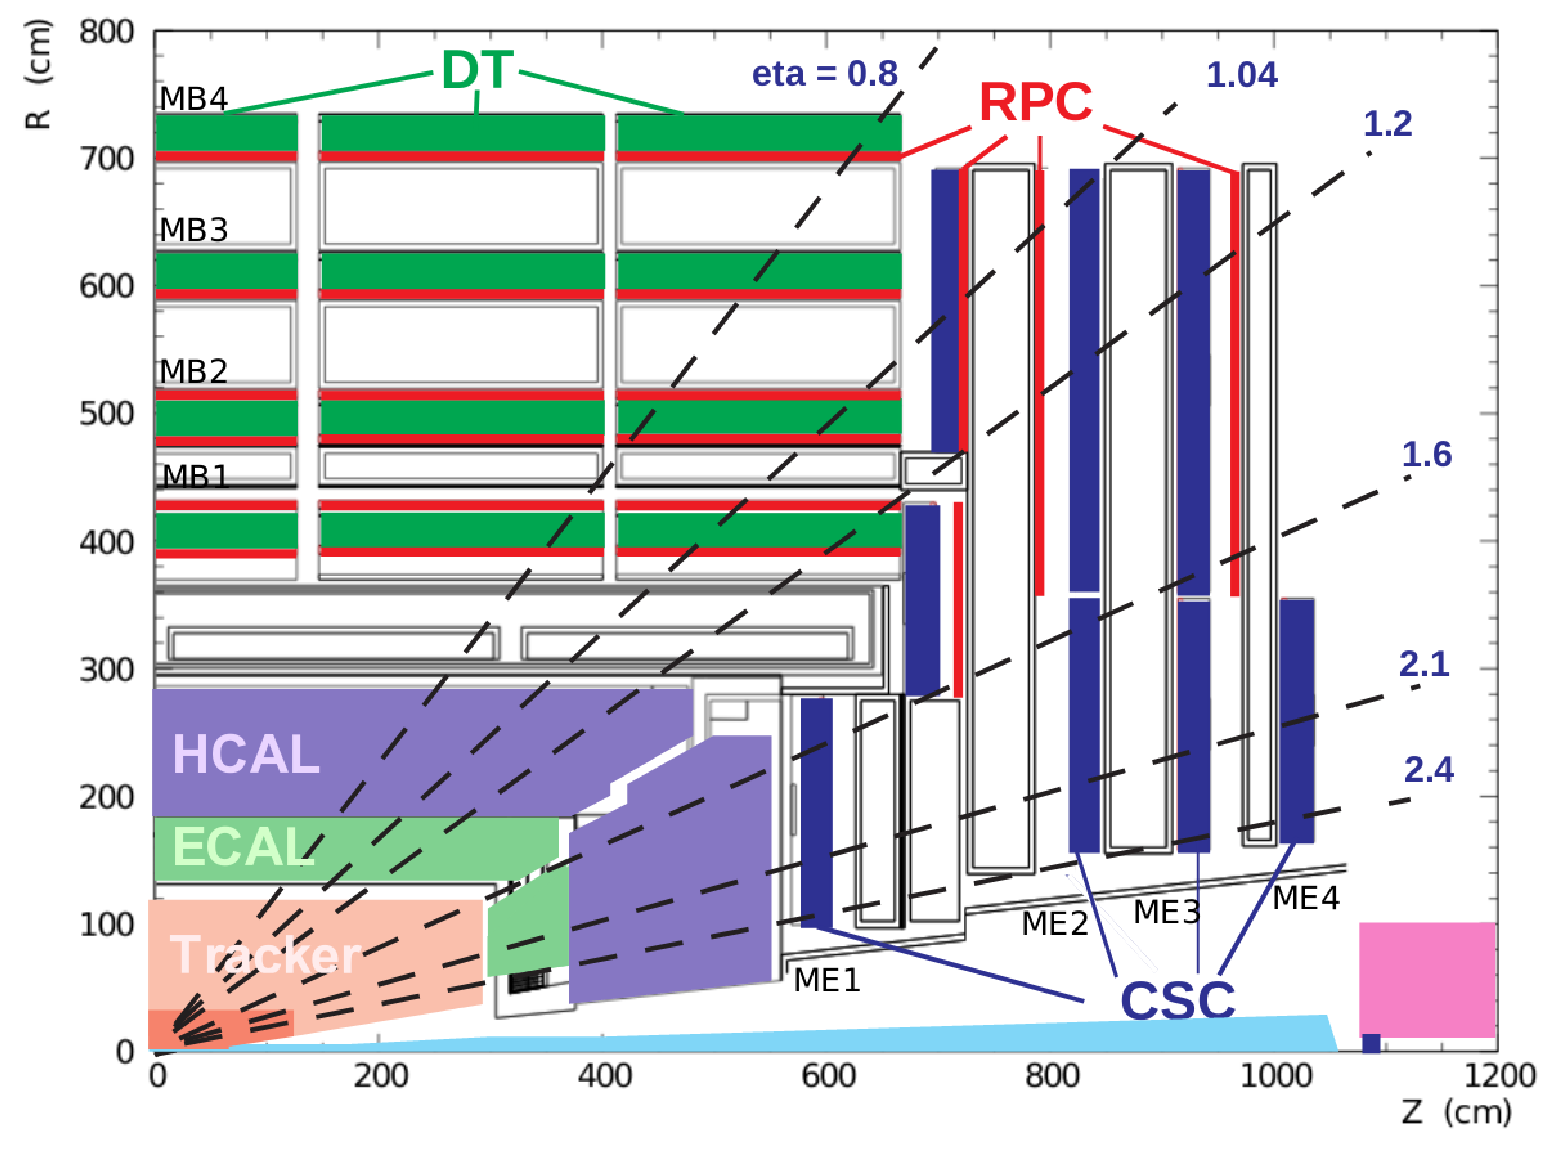
\includegraphics[width=.6\textwidth]{Figures/cms/muon.pdf}
  \caption[The CMS hadronic calorimeter]
  {
    A schematic showing one quarter of the CMS detector. The dashed lines indicate lines of constant pseudorapidity. The locations of the DT, RPC and CSC of the muon tracking system are shown. Figure is taken from in Ref.~\cite{Chatrchyan:2012xi}.
  }
  \label{fig:cms_muon}
\end{figure}

Drift tube (DT) chambers are located in the barrel region, and detect muons for $|\eta|<1.2$, whilst cathode strip chambers (CPS) cover the pseudorapidity range $0.9<|\eta|<2.4$. Both are complimented by a system of resistive plate chambers (RPC) for $|\eta|<1.6$. All rely on gaseous detector technology. As a muon traverses the chamber it ionises gas molecules. The resulting ionisation electrons drift towards the detector's anode producing an electric signal. The choice of detector technology in each region is driven by the properties of the return magnetic field at that point, the rate of muons, and the level of neutron-induced background.

Overall, muons with $p_T$ larger than a few GeV are identified with an efficiency of above 95\%; the corresponding misidentification rate is lower than 1\% for a loose selection and 0.1\% for a tight selection. The momentum resolution for muons with $20<p_T<100$~GeV is between 1.3 and 2.0\% in the barrel ($|\eta|<1.2$) and better than 6\% in the endcaps ($1.2<|\eta|<2.4$). Over this $p_T$ range, the momentum measurement is provided by the silicon tracker. For higher $p_T$ muons, the best momentum measurement is obtained using a combination of information from the silicon tracker and muon chambers, providing a resolution of better than 10\% up to 1~TeV.

\subsection{Trigger}\label{sec:trigger}
The CMS detector operates at a proton bunch crossing frequency of 40~MHz, where each event contains of the order 1~Mb of data~\cite{Khachatryan:2016bia}. A two-tiered trigger system is implemented to manage this high collision rate, selecting only events of interest to be recorded. The Level-1 Trigger (L1T), composed of custom hardware processor boards, successfully reduces the output rate from 40~MHz to 100~kHz. This is compatible with the design read-out rate of the CMS sub-detector electronics~\cite{Sphicas:2002gg}. Selected events are then propagated to the software-based High-Level Trigger (HLT), where more sophisticated algorithms are applied using more detailed event information. The HLT further reduces the event rate to 1~kHz; an acceptable rate to be saved to disk. Crucially, this total reduction in the event rate by a factor of 40,000 is achieved whilst maintaining a high efficiency for the physics processes of interest.

The event detail used in the L1T is limited by the design latency; it must be decided whether to keep or discard an event within a fixed time interval of 4~$\mu$s. As a result, the L1T decision is based on \textit{coarse} measurements of the energy deposited in the calorimeters and muon chambers, and it is currently not possible to use information from the tracker. Simple algorithms are applied to this coarse data, such as the energy sum in an array of ECAL crystals, to decide if the event contains a signature of interest. During the processing time, the full event information is stored in a buffer. Upon reception of a L1T \textit{accept signal}, this full information is read-out and passed to the HLT.

The HLT decision is based on more granular event information, including measurements from the tracker. A single farm of around 1000 commercially-available processors is used, where simplified versions of the full offline reconstruction algorithms are applied to the events. If the event is deemed to be of interest, it is saved to disk and subsequently reconstructed using the full CMS software.

\subsection{Detector summary}
Figure \ref{fig:cms_interactions} illustrates how different objects produced in a p-p collision interact with the CMS detector. Clearly, it is the combination of the different sub-detectors that makes it possible to reconstruct the full range of final-state objects. The CMS approach to object reconstruction is detailed in the following section.

\begin{figure}[htb!]
  \centering
  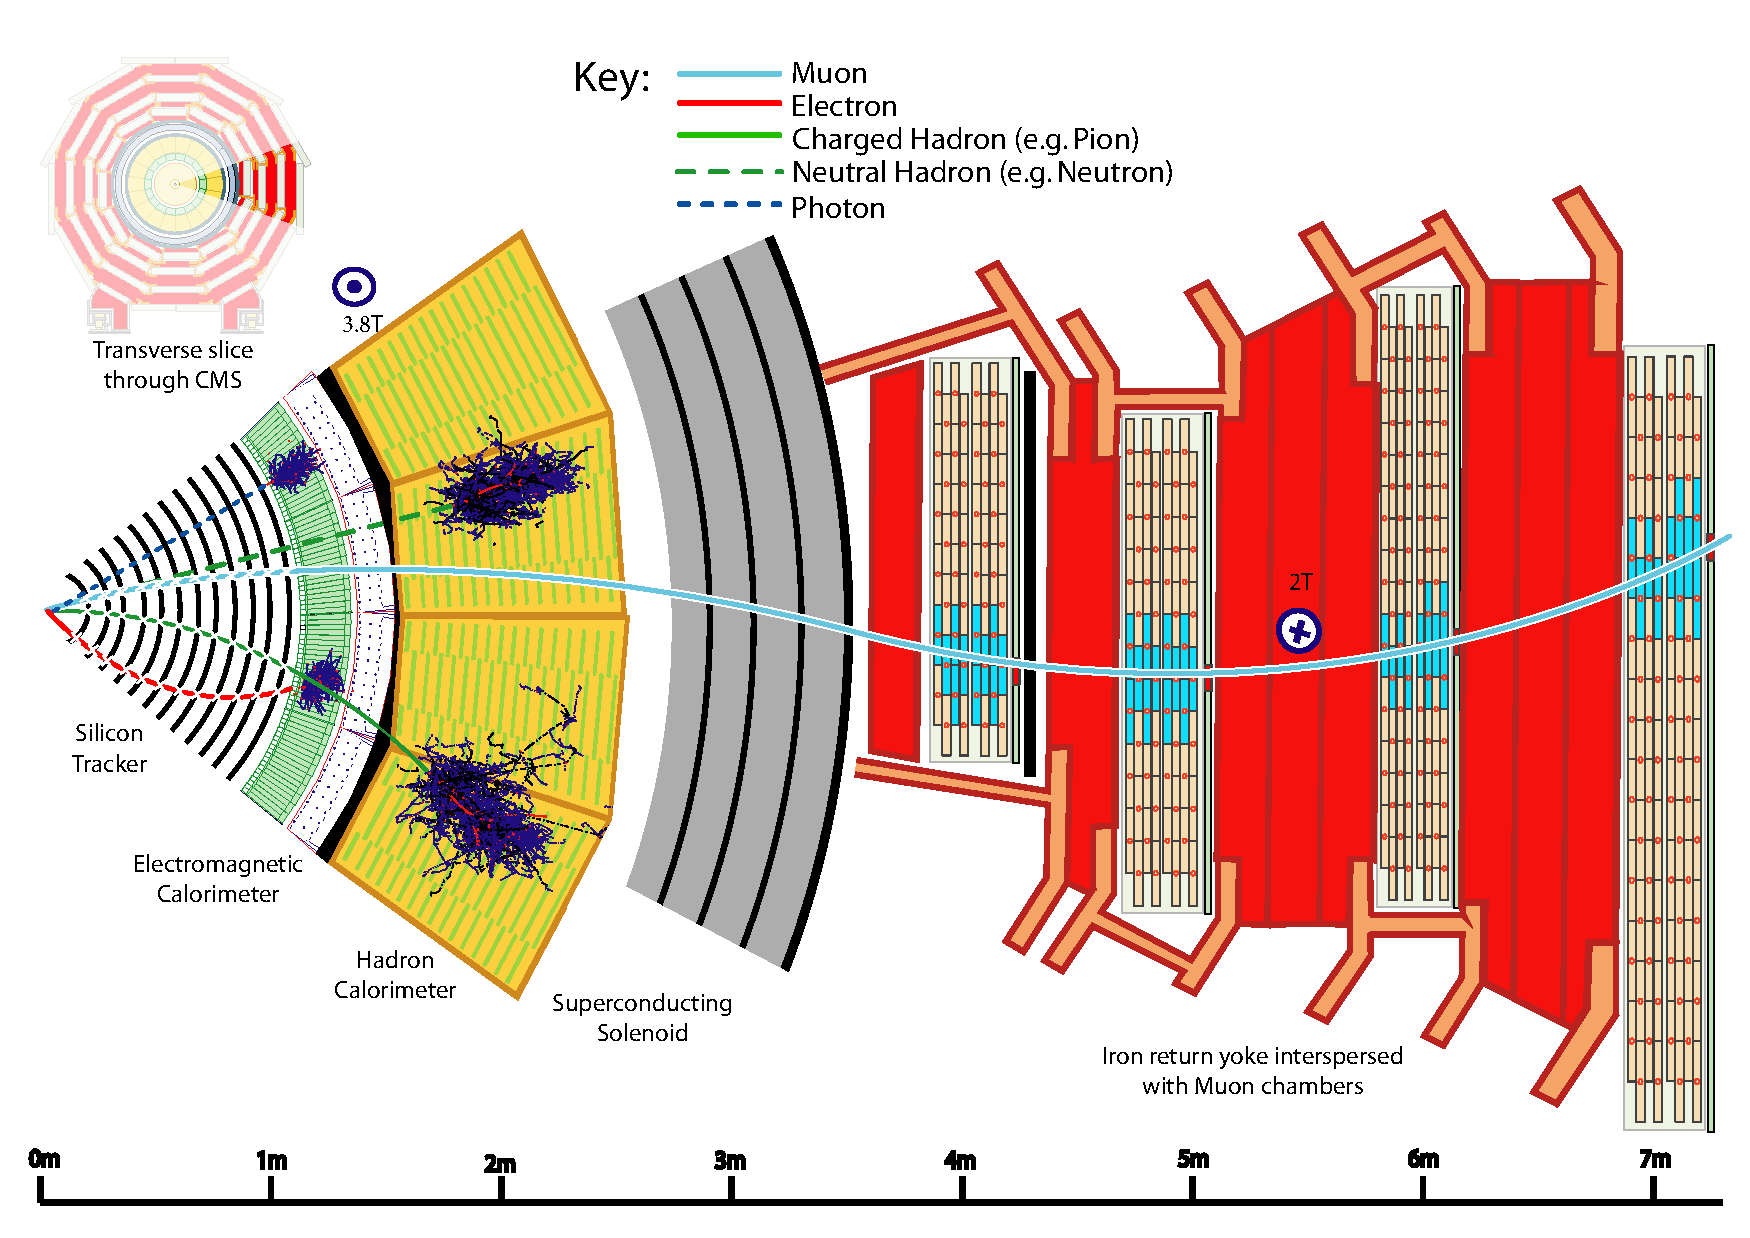
\includegraphics[width=1\textwidth]{Figures/cms/CMS-PRF-14-001_Figure_001.pdf}
  \caption[Particle interactions in the CMS detector]
  {
    A transverse slice of the CMS detector. The diagram illustrates the typical interactions of multiple final-state objects, produced at the interaction point (furthest left), with the various CMS sub-detectors. Charged particles, such as electrons, muons and charged hadrons, are deflected by the solenoidal field and leave hits in the silicon tracker. Electrons and photons create electromagnetic showers in the ECAL, whilst charged and neutral hadrons produce hadronic showers in the HCAL. Muons traverse through the detector, are deflected in the opposite direction by the return magnetic field, and leave hits in the muon chambers. Figure is taken from Ref.~\cite{Sirunyan:2017ulk}.
  }
  \label{fig:cms_interactions}
\end{figure}

\section{Object reconstruction: particle flow}\label{sec:particle_flow}
CMS adopts a holistic approach to event reconstruction: the information from all subdetectors is correlated to identify each final-state particle, and the corresponding measurements are combined to reconstruct the particle properties based on this identification~\cite{Sirunyan:2017ulk}. The comprehensive list of final-state particles produced by the algorithm then enters physics analyses. This approach, referred to as the \textit{Particle-Flow} (PF) reconstruction, provides a global event description and offers unprecedented performance in terms of jet and \met reconstruction, and electron and muon identification. Furthermore, objects produced from pileup interactions can be identified efficiently, enabling powerful pileup mitigation.

The basic elements of the PF reconstruction are \textit{tracks} in the silicon tracker and muon systems, and \textit{clusters} of energy in the ECAL and HCAL. Tracks are built using a combinatorial track finder algorithm~\cite{Chatrchyan:2014fea}, that proceeds in the following way:
\begin{itemize}
    \item An initial track candidate (seed) is identified as a few (2-3) hits in the tracker, from which the initial trajectory parameters and their corresponding uncertainties are calculated.
    \item A Kalman filter~\cite{BILLOIR1990219} based track finder is applied: the expected flight path of a charged particle is extrapolated from the seed trajectory parameters, where additional hits along this path are assigned to the track candidate. Following this, a track-fitting module is used to calculate the trajectory parameters more precisely.
    \item The track candidate is accepted or rejected based on a set of quality criteria.
\end{itemize}
\noindent
This is repeated for six iterations, in a process referred to as \textit{iterative tracking}. The initial iterations locate the most prominent tracks, for example those with high $p_T$ and lying close to the IP. After each iteration, hits associated with a track are removed from the process, and the quality criteria for forming seeds and building tracks are relaxed. Subsequent iterations then locate a more difficult class of tracks with low $p_T$ and/or high displacement, in a less combinatorial-complex environment. Ultimately, this iterative procedure helps to increase the tracking efficiency, whilst keeping the misreconstructed track rate to a reasonable level. An additional procedure is used to build muon tracks from hits in the muon chambers~\cite{Chatrchyan:2012xi}.

Clusters are built by collecting the energy deposits in the calorimeters using a dedicated clustering algorithm~\cite{Khachatryan:2015hwa}. The procedure is effectively the same for the ECAL and HCAL, but is introduced in the context of a photon shower in the ECAL here:
\begin{itemize}
    \item A seed crystal is identified as a local energy maximum, above a given energy threshold.
    \item Clusters are built iteratively around the seed. This is done by aggregating crystals which share at least one corner in common with a crystal already in the cluster, and have an energy in excess of twice the noise level of the ECAL.
    \item If a given crystal can belong to multiple clusters, the crystal energy is shared between them assuming a Gaussian shower profile.
    \item Photons that convert to $e^+e^-$ pairs in the tracker, typically have a wider shower profile. This results from the bending of the electrons/positrons in the solenoidal field, which radiate bremsstrahlung photons and thus deposit energy over a wide azimuthal ($\phi$) range. Superclusters (SC) are built by merging together clusters. This ensures good containment of the electromagnetic shower for converting photons. The spatial position of the SC ($\eta$,$\phi$) is defined as the logarithmic energy-weighted average position of the individual crystals. The SC energy reconstruction was previously discussed in section \ref{sec:cms_ecal}.
\end{itemize}
\noindent
The procedure for reconstructing photon and electron showers in the ECAL is identical. This is an important feature of the \Hgg analysis described in chapters \ref{chap:hgg_overview}-\ref{chap:hgg_results}, as it allows the use of \Zee events for the photon energy calibration and for the validation of numerous multivariate algorithms.

A given final-state particle can give rise to several tracks and clusters in the various CMS subdetectors. The dedicated \textit{link algorithm} is applied to connect these basic PF elements and output a PF candidate from the following classes:
\begin{itemize}
    \item \textbf{Muons}: identified as a track in the muon chambers linked to a track in the tracker. Energy is calculated from the track curvature.
    \item \textbf{Electrons}: identified as an ECAL SC linked to a track in the tracker. Energy is calculated from a combination of the track curvature and the SC energy. 
    \item \textbf{Photons}: identified as an ECAL SC with no associated track in the tracker. Energy is calculated from the SC energy only.
    \item \textbf{Neutral hadrons}: identified as linked clusters in the ECAL and HCAL, with no associated track in the tracker. Energy is calculated as the sum of cluster energies.
    \item \textbf{Charged hadrons}: identified as linked clusters in the ECAL, HCAL, and a track in the tracker. Energy is calculated from a combination of the track curvature and the sum of cluster energies.
\end{itemize}
\noindent
Collections of PF candidates are then used in CMS physics analyses. Chapter \ref{chap:hgg_overview} details how they are used in the \Hgg analysis

\section{Simulating hadron collisions}\label{sec:mc}
The goal of the CMS experiment is ultimately to use the final state objects in the detector to infer some knowledge on the parameters of the model Lagrangian, $\vec{\alpha}$. This could be, for example, the mass of the Higgs boson, the couplings of the Higgs boson to other SM fields, or even the Wilson coefficients of an EFT. We can establish a likelihood function~\cite{Brehmer:2020cvb} which quantifies the probability of observing an event, x, given the model parameters, $\vec{\alpha}$,

\begin{equation}\label{eq:mc_integral}
    L(x\,|\,\vec{\alpha}) = \int {\rm{d}}z_d \int {\rm{d}}z_s \int {\rm{d}}z_p \, p(x|z_d)p(z_d|z_s)p(z_s|z_p)p(z_p|\vec{\alpha}),
\end{equation}

\noindent
where $x$ is a vector of observables such as the reconstructed energies, momenta, and angles of all final state objects. The latent variables, $z_i$, are defined as follows:
\begin{itemize}
    \item $z_p$: the four-momenta, charges and helicities of the partons in the hard scattering event. The quantity $p(z_p|\vec{\alpha})$, which defines the probability for partons, $z_p$, given the model parameters, $\vec{\alpha}$, is related to the squared hard-scattering matrix element, $|\mathcal{M}|^2$. The collection of incoming and outgoing partons is referred to as the \textit{parton-level} event.
    \item $z_s$: encodes the entire shower history of the partons. Effectively, $p(z_s|z_p)$ describes the transition from the parton-level event, $z_p$, to the \textit{particle-level} event, $z_s$.
    \item $z_d$: describes the interactions of the particles with the detector, such that $p(z_d|z_s)$ describes the probability of observing a set of electronic signals in the detector given the particles, $z_s$. This is not a simple problem; the CMS detector has around $10^8$ read-out channels. The final term, $p(x|z_d)$, explains how the detector signals are reconstructed into the final state objects (section \ref{sec:particle_flow}).
\end{itemize} 

The sheer complexity of the problem is illustrated in Figure~\ref{fig:mc_illustration}. Clearly, evaluating the integral of equation~\ref{eq:mc_integral} over the full parameter space is impossible: we cannot simply take the observed events, $x$, and the model parameters, $\vec{\alpha}$, and compute the likelihood, $L(x\,|\,\vec{\alpha})$. Consequently, the likelihood is said to be \textit{intractable}.

\begin{figure}[htb!]
  \centering
  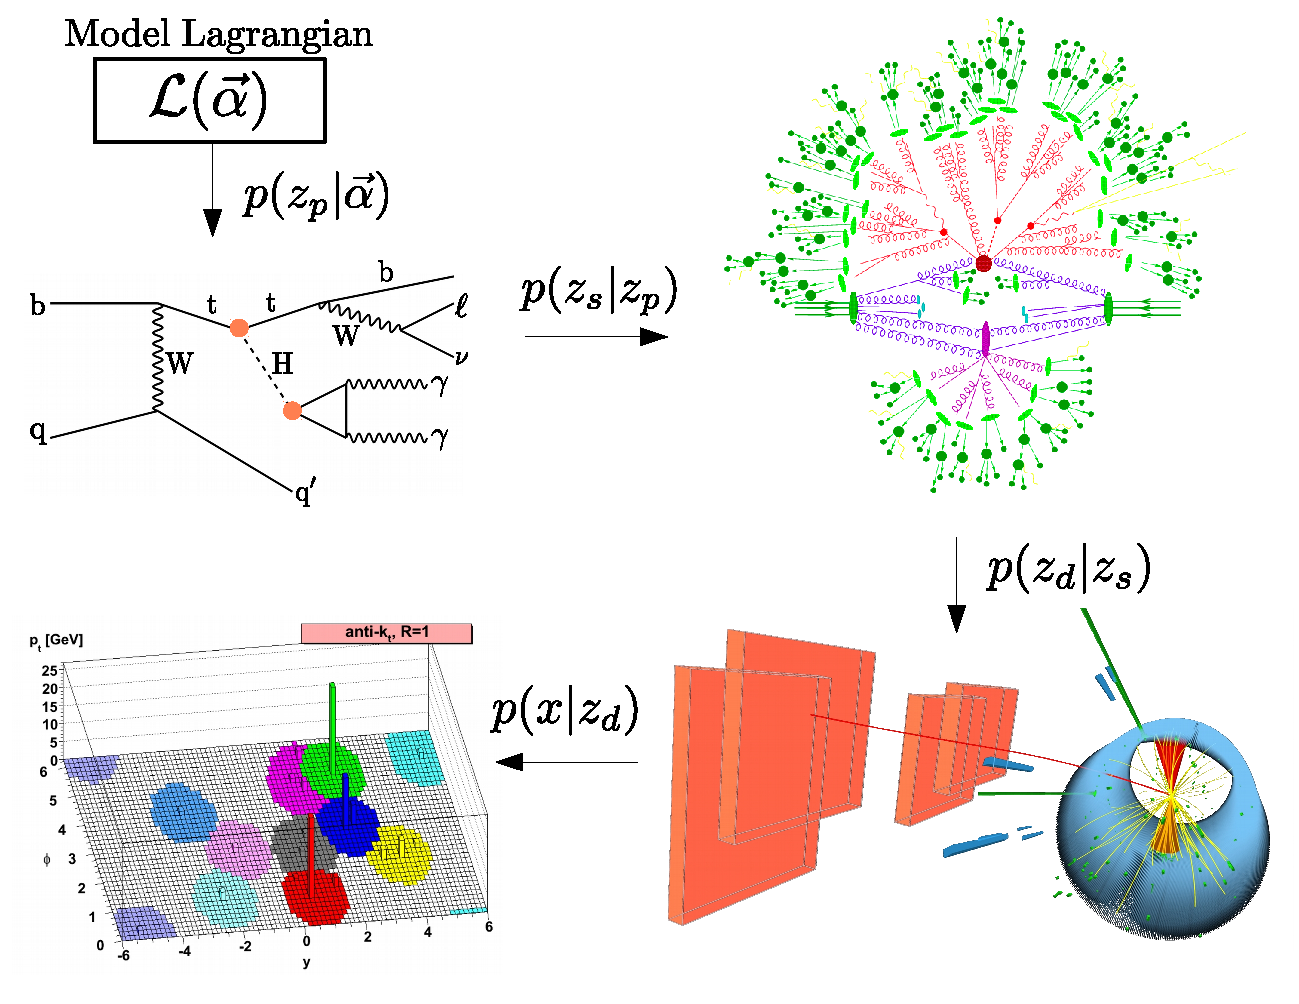
\includegraphics[width=.8\textwidth]{Figures/cms/mc_integral.pdf}
  \caption[The intractable likelihood function of the CMS experiment]
  {
    An illustration of the intractable likelihood function of the CMS experiment. The Feynman diagram (top right) corresponds to tHq production in the \Hgg decay channel, in which the top quark decays leptonically. The event display (bottom right) corresponds to a candidate tHq, \Hgg event in the CMS detector, adapted from the additional material of Ref.~\cite{CMS-PAS-HIG-19-015}. The parton shower diagram (top right) and the and anti-$k_T$ algorithm illustration (bottom left) are taken from Refs~\cite{Hoche:2014rga} and \cite{Cacciari:2008gp}, respectively.
  }
  \label{fig:mc_illustration}
\end{figure}

To overcome this experimental challenge, we approximate the integral using a series of state-of-the-art Monte Carlo (MC) simulators. Firstly, the MC generation chain begins with simulating the hard scattering process. This models the distribution of initial state partons inside the colliding protons, computes the relevant matrix element, $\mathcal{M}_{i\rightarrow f}$, for certain values of the input model parameters, $\vec{\alpha}$, and generates parton-level final states with some probability. Following this, the parton shower is simulated, where initial and final state coloured partons are showered and formed into hadrons, and any remaining unstable particles (e.g. $H$, $W^{\pm}$, etc.) are decayed. Additional secondary interactions to the hard scattering process are modelled as underlying events. Finally, the events are propagated through a simulation of the CMS detector, where the response of the detector is calibrated to match the performance and efficiency observed in data. The final output of this chain is a collection of generated collision events which aims to match real events in data as closely as possible. Ultimately, we can then compare the MC simulation to data to infer knowledge on the model Lagrangian parameters, $\vec{\alpha}$.

MC simulation is used in many ways in this thesis, most notably for the SM simulation of events in the \Hgg analysis (section \ref{sec:hgg_simulation}), and for deriving the EFT parametrisation of Higgs boson cross sections and decay widths (section~\ref{sec:eft_parametrisation}). The remainder of this section will help the reader understand some of the key concepts of MC event generation that are discussed throughout.

\subsubsection{Factorisation and renormalisation}
Two of the main theoretical aspects of the MC simulation are factorisation and renormalisation. Factorisation concerns the decoupling of the long-timescale (low energy) physics from the short-timescale (high energy) hard scattering process, such that the different energy regimes can be simulated separately~\cite{doi:10.1146_annurev.nucl.55.090704.151505}. A factorisation scale, $\mu_F$, is introduced to avoid IR divergences in the hard scattering calculation. This scale effectively defines the borderline between the low energy and high energy physics.

Renormalisation details the regularisation of UV divergences at the opposite end of the energy range~\cite{Brock:1993sz}. These arise due to the unrestricted integration of the momentum flow through internal loops in the Feynman diagrams. Regularisation gives rise to a renormalisation scale, $\mu_R$, which acts as an UV cut-off. The bare couplings of the theory absorb all the very short-timescale physics beyond this cut-off, and as a consequence, acquire a $\mu_R$ dependence. For example, in QCD the contribution of quarks and gluons in loops is absorbed into the strong coupling constant, which runs according to,
\begin{equation}
    \alpha_s(Q^2) = \frac{\alpha_s(\mu_R^2)}{1+\frac{\beta_0}{4\pi}\,\alpha_S(\mu_R^2)\,\ln\Big(\frac{Q^2}{\mu_R^2}\Big)},
\end{equation}

\noindent
where $Q^2$ represents the energy scale of the process. The constant $\beta_0$ is positive ($>0$), which confirms the notion of \textit{asymptotic freedom}~\cite{PhysRevLett.30.1343}: the strength of $\alpha_s$ decreases ($\alpha_S(Q^2) \rightarrow 0$) as the energy scale increases ($Q^2\rightarrow\infty$). At very high scales, the strongly-interacting partons can be treated as independent particles. 

Crucially, the underlying physics does not depend on these scales: $\mu_R$ and $\mu_F$. They are simply an artifact of using perturbation theory to calculate the process, and truncating the expansion to a particular number of terms. Nevertheless, there exists a freedom in the choice of their values, where some choices can be better than others. Since we know an observable (e.g. a cross section) should not depend on $\mu_R$ and $\mu_F$, it is theoretically favourable to choose values where the observable varies least with the scales. This is typically of the order of the energy scale characterising the process (e.g. $\mu_R = m_Z$ for Z-pole measurements) to avoid large logarithmic terms in the perturbative expansion~\cite{Buckley:2011ms}. The theoretical uncertainty originating from the series truncation can then be modelled by varying the scales about their nominal value, usually by a factor of two~\cite{doi:10.1146_annurev.nucl.55.090704.151505}.

\subsubsection{Parton distribution function}
Parton distribution functions (PDFs), $f_{i}(x,\mu_F)$, model the number density of parton type, $i=\{g,u,d,s,c,(b)$,+anti-quarks$\}$, with momentum fraction, $x$, inside the colliding proton. These functions effectively absorb the long-timescale physics of the internal proton, and therefore acquire a dependence on the factorisation scale, $\mu_F$. The exact forms of the PDFs are extracted using data from lepton-hadron and hadron-hadron collisions, and are defined in so-called PDF sets to be used by the MC generators~\cite{Butterworth:2015oua}. The evolution of the PDF with increasing $\mu_F$ is modelled with the DGLAP equations~\cite{Gribov:1972ri,Dokshitzer:1977sg,Altarelli:1977zs}. Ultimately, the choice of PDF affects not only the simulation of the hard scattering, but also the parton showering and the modelling of multiple parton interactions in the underlying event. This influences both the predicted cross sections and the event kinematics.

\subsubsection{Parton-level event generation}
The fully differential cross section for a hard scatter process ($a,b \rightarrow f$) in a hadron collision is calculated by factorising the initial state physics from the hard scatter, according to~\cite{ellis_stirling_webber_1996},
\begin{equation}\label{eq:cross_section_calc}
    \frac{{\rm{d}}\sigma}{{\rm{d}}\Phi_n} = \sum_{a,b} \int^1_0 {\rm{d}}x_a {\rm{d}}x_b f_a(x_a,\mu_F) f_b(x_b,\mu_F) \times \frac{1}{\hat{s}}|\mathcal{M}_{a,b\rightarrow f}|^2(\Phi_n;\mu_F,\mu_R,\vec{\alpha}),
\end{equation}
\noindent
where $\Phi_n$ represents the final-state phase space, $|\mathcal{M}_{a,b\rightarrow f}|^2$ is the squared-matrix element averaged over the initial state spin and colour degrees of freedom, and $1/\hat{s}=1/2x_ax_bs$ is the initial state parton flux, where $s$ is the squared hadronic centre-of-mass energy. As introduced above, the factorisation is possible since the hard scatter occurs over a very short timescale (high energy), whilst the interactions within the proton occur over much longer timescales (low energy). This means that when computing the hard scatter process, we can assume the dynamics within the proton are static and treat the initial state partons, $a$ and $b$, as independent. As a result, we can use perturbation theory to calculate hard scatter matrix elements, as described in the following section.

In the parton-level event generation, events are sampled from the initial and final-state phase spaces, and a probability is assigned according to equation~\ref{eq:cross_section_calc}. By generating large numbers of events, we can successfully build up the kinematic distributions that one would expect to see in data (for some values of the model parameters, $\vec{\alpha}$). A cross section, $\sigma^i$, for a particular region of the final state phase space, $\Phi^i_n$ can then be inferred by integrating equation~\ref{eq:cross_section_calc} over this region. In the STXS framework, the regions are defined according to the bin boundaries introduced in section~\ref{sec:theory_stxs}.

\subsubsection{Order in perturbation theory}
The hard scatter is defined by a high momentum transfer, $Q^2$, and as a result the strong coupling constant, $\alpha_s(Q^2)$, is small. The perturbative expansion of the matrix element, $|\mathcal{M}_{a,b\rightarrow f}|^2(\Phi_n;\mu_F,\mu_R,\vec{\alpha})$, can therefore be performed in powers of $\alpha_s$, which is done up to some finite order in the calculation. This can be pictured in terms of Feynamn diagrams,
where going to higher orders equates to including diagrams with additional internal loops. The leading order (LO) calculation corresponds to including only the first term in the expansion. The subsequent orders are referred to as next-to-leading order (NLO), next-to-next-to-leading order (NNLO) and so on. For example, the inclusive ggH cross section has been calculated at N$^{3}$LO~\cite{Anastasiou:2016cez}.

As described earlier, the neglection of higher-order terms introduces some intrinsic uncertainty into the calculation. We model this uncertainty by varying the renormalisation and factorisation scales, $\mu_R$ and $\mu_F$, by a factor of two around the nominal scale values.
Ultimately, the more terms that are included in the perturbative expansion (going to a higher order), the less the predictions depend on the scales, or in other words, the accuracy of the predictions increases.

\subsubsection{Parton shower and hadronisation}
Parton showering describes the evolution in momentum transfer from the hard scattering process at high scales, to the formation of the final-state hadrons at low scales, typically $\mathcal{O}(1$~GeV). The evolution is performed by modelling the QCD radiation of initial state and final state coloured partons using perturbative QCD~\cite{Buckley:2011ms}. The radiated gluons can go on to radiate further, producing additional gluons and quark-antiquark pairs, which are typically soft or collinear with the outgoing partons. In this manner, the parton shower effectively \textit{dresses} the event with additional QCD radiation, which is iterated until the momentum transfer reaches the scales associated with hadron formation. Free parameters of the parton showering model are tuned to improve the description of real data, where different values of these parameters are referred to as different parton shower tunes~\cite{Khachatryan:2015pea,Sirunyan:2019dfx}.

Hadronisation occurs at the end of the parton shower, and describes the confinement of the outgoing coloured partons into colourless hadrons. At this energy scale, QCD becomes strongly interacting and perturbation theory breaks down. Dedicated hadronisation models have been developed to deal with this non-perturbative regime, such as the string fragmentation and cluster models~\cite{Andersson:1983ia,Andersson:1998tv,Amati:1979fg}. Fortunately, the hadronisation process can be effectively decoupled from the upstream hard scatter process, and therefore once tuned, the hadronisation model can be applied successfully to different physics processes at different energies~\cite{Buckley:2011ms}.

\subsubsection{Jets}
The final state objects in hadron collisions typically include collimated sprays of hadrons, referred to as jets. These originate from the parton showering and hadronisation of both final state partons and the QCD radiation of initial state partons. Jets are not fundamental objects defined by theory, and as a consequence, they must be defined according to some jet algorithm~\cite{Salam:2009jx}. These algorithms associate which hadrons belong to which jet according to some set of rules, and then reconstructs their total momentum. One such example used in this thesis is the anti-$k_T$ algorithm, which repeatedly combines pairs of particles according to some specified distance measure~\cite{Cacciari:2008gp}.

Jets can originate from both the hard scatter matrix element and the parton shower, where the former is more accurate for modelling harder (high momentum) jets and the latter for softer (low momentum) jets. When combining the two approaches a double-counting occurs, leading to an overestimation of the jet multiplicity in an event. This is avoided by applying a jet matching or merging procedure~\cite{Alwall:2007fs}. These typically introduce some cut-off merging scale, above which the event uses jets originating from the matrix element, and below which jets originating from the parton shower are used.

\subsubsection{Underlying event}
Secondary QCD interactions occur in each hadron collision in addition to the hard scattering process. The additional activity which is not associated with the hard interaction is referred to as the underlying event~\cite{Buckley:2011ms}. These interactions typically involve coloured particles, which can ``talk" to the particles in the hard scattering. As a result, the underlying event can influence the properties of the process of interest. Like the parton shower, the free parameters of the underlying event model are tuned to match what is observed in data. 

\subsubsection{Detector simulation}
The particle-level events are propagated through a simulation of the CMS detector. This is typically done using the \textsc{Geant4} package~\cite{Agostinelli:2002hh} which models the geometry of each subdetector, and describes how particles traverse through the CMS solenoidal field and subsequently interact with the detector material. The outputs are hits (deposits of energy) in the various subdetectors, which have been designed to match the true electronic read-out channels of the detector. Consequently, we can apply the same event reconstruction techniques on the MC simulation as to what is used on data. 

To accurately model the detector response in terms of the efficiency and reconstruction performance, the detector simulation must be calibrated. This typically involves using a set of measurements e.g. the jet momentum distribution, and tuning the simulation to match what is observed in data. A mis-modeling of the detector response introduces (experimental) systematic uncertainties into the analysis. For example, in the context of the \Hgg analysis, the mis-modeling of the photon energy resolution will affect the predicted signal shape, and consequently the extracted results. Therefore, there is an extensive programme of work in the CMS experiment that concerns the calibration of the detector simulation to match data.

It is worth introducing some terminology at this stage. Throughout this thesis, \textit{truth-level} quantities correspond to the event properties in the simulation before the detector modelling i.e. their true values. These are the quantities which are used in the STXS event classification into the different bins. On the other hand, \textit{reconstruction-level} quantities refer to the event properties after the detector. For example, the Higgs boson transverse momentum, $p_T^H$, is a truth-level quantity, whilst the transverse momentum of reconstructed photon pair, $p_T^{\gamma\gamma}$, is the equivalent reconstruction-level quantity. The difference between the two is purely a result of the detector efficiency and resolution. As discussed at the beginning of this section, the ultimate goal of the experiment is to infer knowledge about the parameters of the model lagrangian. In the context of STXS measurements, this requires unfolding the response of the detector, or in other words using the reconstruction-level information to infer the truth-level event information.

\subsubsection{Generators}
A number of tools are used to perform the different stages of MC event generation. In this thesis, the \textsc{MG5\_aMC@NLO}~\cite{Alwall:2014hca}, \textsc{Powheg}~\cite{Nason:2004rx,Frixione:2007vw,Alioli:2008tz,Nason:2009ai,Alioli:2010xd,Hartanto:2015uka} and \textsc{sherpa}~\cite{Gleisberg:2008ta} generators are used to simulate the parton-level event. This includes the modelling of the PDFs and the computation of the hard scattering matrix element to some fixed order in the perturbative expansion. The generators are typically interfaced with \textsc{Pythia8}~\cite{Sjostrand:2014zea} for parton showering and hadronisation. Finally, the \textsc{Geant4} and \textsc{Delphes} packages are used to performed a detailed and fast simulation the CMS detector, respectively.

\section{ML algorithms}\label{sec:ml_algo}
Machine learning (ML) algorithms have become a widely used tool in high energy physics. This is particularly true for the \Hgg analysis described in chapters~\ref{chap:hgg_overview}--\ref{chap:hgg_results}, where ML algorithms are used for a number of tasks including the photon energy regression and the event categorisation. Because of this, it is worth spending some time introducing the concept of ML. 

The field of machine learning concerns developing sophisticated algorithms with the ability to \textit{learn} from data, and subsequently apply the learnt information to solve complex problems. A generic ML problem can be formulated as follows~\cite{hastie01statisticallearning}. The data are expressed as a vector space of dimension $m$: $X = \mathbb{R}^m$, where each dimension corresponds to an observable quantity referred to as a \textit{feature}. An element of the data set, for example an event in a event classification task or a SC in an energy regression task, corresponds to a single feature vector, $\vec{x} \in X$. The full data set of $N$ elements is defined by the set of feature vectors, $\vec{x}_i$, where $i=1,...,N$. The purpose of the ML algorithm is to develop a model,

\begin{equation}
    f(\vec{x}\,|\,\vec{w}) \rightarrow Y,
\end{equation}

\noindent
to \textit{predict an outcome}, $Y$, based on the feature vector, $\vec{x}$, given a set of model parameters, $\vec{w}$. We can identify two main types of ML algorithm based on the form of the predicted outcome:

\begin{itemize}
    \item A \textit{classification task} equates to predicting one of $k$ possible \textit{output classes}: $f(\vec{x}\,|\,\vec{w})\rightarrow y$, where $y\in \{1,...,k\}$. The obvious example here is a binary signal-vs-background event classifier, which aims to predict if an event looks signal-like or background-like based on a set of kinematic features. Many classification algorithms are introduced throughout this thesis, including the HGCAL L1T algorithm introduced in section~\ref{sec:egid}.
    
    \item A \textit{regression task} equates to predicting a quantitative outcome, or in other words a continuous value: $f(\vec{x}\,|\,\vec{w})\rightarrow y$, where $y\in \mathbb{R}$. An example in this thesis is the SC energy regression described in section \ref{sec:photon_reconstruction}, where the regressor predicts the true energy of the SC (and its uncertainty) using a combination of shower shape, seed crystal, and pileup-related features.
\end{itemize}

There are two stages when developing an ML algorithm. The learning process is referred to as \textit{training} the model, where the values of the model parameters, $\vec{w}$, are optimised to maximise the performance. Following this, the performance of the model is evaluated using so-far unseen data; this is referred to as the \textit{testing} stage.

A loss function, $L$, is constructed to measure the performance of the model, $f$, for a given set of input features, $\vec{x}$:
\begin{equation}
    L[\,f(\vec{x}\,|\,\vec{w})\,] \rightarrow \mathbb{R}.
\end{equation}
\noindent
\textit{Supervised} learning algorithms refer to the case where the target values, $y$, are known for each element of the training data set, $\vec{x}$. In this case, the loss function is constructed to minimise the discrepancy between the true and estimated values of the outcome, $y$. An additional class of algorithms where the target values are not known are referred to as \textit{unsupervised} learning algorithms~\cite{10.5555/3086952}; these do not feature in this thesis and are therefore not described further. Learning effectively corresponds to reducing the value of $L$ by optimising the parameters, $\vec{w}$. In practice, for most ML algorithms this consists of some gradient based optimisation, where one descents the gradient of $L$ with respect to $\vec{w}$ in order to find the minimum,
\begin{equation}\label{eq:loss_minimum}
    \vec{\nabla}_{\vec{w}}\,L = 0.
\end{equation}
\noindent
It is often not viable to evaluate this expression over the entire training dataset, especially in the case of large statistics with a high number of input features (dimensionality). A number of powerful optimisation algorithms have been developed to combat this~\cite{10.5555/3086952,pmlr-v28-sutskever13,kingma2017adam}. These typically involve calculating the gradient for small batches of training data and optimising $\vec{w}$ iteratively, and extending this with the concept of \textit{momentum}, where the update to the parameter vector, $\vec{w}$, depends on the size of the gradient at that point.

Crucially, it is not sufficient to simply find the configuration of $\vec{w}$ which minimises the loss for the training data set. In addition, the model is also required to generalise to new data. Therefore, the performance is evaluated on an independent test set, which is chosen to be representative of the whole data set. If the performance is significantly degraded for the test set, then the model is said to have \textit{over-trained} and has become specific to properties of the training set. One approach to controlling the level of over-training is to introduce regularisation terms into the loss function~\cite{10.5555/3086952}.

A large variety of ML algorithms are used in high energy physics. In this thesis, the most commonly used is the Boosted Decision Tree (BDT) algorithm~\cite{Yang_2005}, which is described in the remainder of this section. Neural networks are also used for discriminating between the ttH and tH production modes in the \Hgg event classification (section \ref{sec:event_categorisation}), as well as for identifying jets originating from the decay of b quarks (section \ref{sec:hgg_otherobjects}); further detail concerning neural networks can be found in Refs.~\cite{hastie01statisticallearning,10.5555/3086952,bishop:2006:PRML}.

BDTs are an example of \textit{ensembling}, where multiple models are trained (base learners) and combined in some way to improve the overall performance of the algorithm. The base learners in this case are Decision Trees (DT)~\cite{Quinlan86inductionof}, which are built according to the following procedure:

\begin{itemize}
    \item The feature space is partitioned into regions according to some selection (cut) on one or more of the input features. The choice and position of the cut is optimised according to a measure of purity for classification tasks, or a loss function such as the mean-squared error for regression tasks.
    
    \item This partitioning is repeated in each region, creating further subregions based on a new, optimised selection cut.
    
    \item The procedure terminates when a stopping criterion is reached. This can either be due to a predefined \textit{max depth} (maximum number of splittings), or when a particular value of the splitting quantity (e.g. purity) has been reached. The final regions of the feature space that are not further split are referred to as \textit{leaves}. Each leaf is assigned an output value according to the data points in that region: for classification, this is the most common output class; for regression, this is the mean of the data values.
    
    \item DTs are regularised by \textit{pruning} branches which use unimportant features and give no performance improvement. This help mitigate over-training.
\end{itemize}

An ensemble of DTs is then constructed using a \textit{boosting algorithm}~\cite{10.1214/aos/1024691079,10.1214/aos/1013203451}. Here, multiple DTs are trained in succession, where each iteration aims to improve upon the weaknesses of the previous base learners. The final ensemble (BDT) is defined as a weighted linear combination of the individual DTs, $f_j(\vec{x}\,|\,\vec{w}_j)$, with corresponding selection cuts, $\vec{w}_j$, according to,
\begin{equation}
    F(\vec{x}\,|\,\vec{\gamma},\vec{w}) = \sum^{N_{\rm{DT}}}_j \gamma_j \cdot f_j(\vec{x}\,|\,\vec{w}_j).
\end{equation}
\noindent
The set of coefficients, $\vec{\gamma} = (\gamma_1,...,\gamma_{N_{\rm{DT}}})$, are determined by the boosting algorithm. Building an ensemble, $F$, in this way produces a more powerful predictor and helps to overcome the disadvantages of individual DTs. One important consequence for classification tasks is the BDT outputs are no longer restricted to discrete values, but become continuous variables representing the output class probabilities. For a binary signal-vs-background classifier, a value close to 1 corresponds to a signal-like event, whereas a value close to -1 corresponds to a background-like event. Selection criteria on these so-called \textit{output scores} are a common feature of the \Hgg analysis in chapter \ref{chap:hgg_overview}. 

\section{Summary}
This chapter has introduced the CMS experiment at the Large Hadron Collider. After briefly describing the CERN accelerator complex in section \ref{sec:lhc}, the various subsystems of the CMS detector were explained in section \ref{sec:cms}, namely the tracker, ECAL, HCAL, muon chambers, and the trigger system. Here, particular attention was given to the the energy reconstruction of photon showers in the ECAL, as the photon energy resolution drives the sensitivity of the \Hgg analysis described in the next chapters. Following this, the chapter shifted focus to a number of general techniques used in CMS physics analyses. Section \ref{sec:particle_flow} provided an introduction to the reconstruction of final state objects in the CMS detector using the Particle Flow algorithm. Monte-Carlo simulations of collision events were described in section \ref{sec:mc}. Finally, the chapter concluded with a general description of ML algorithms, which become a recurrent tool throughout the course of this thesis.